\section{Como Construído}

\begin{frame}{Preparação do sinal de áudio corrompido}
	O sinal de áudio conterá:
	\begin{itemize}
	    \item Voz;
	    \item Ruído Branco limitado à faixa de 300 Hz em trono de 2 kHz
	\end{itemize}
	    \begin{figure}[!htb]
        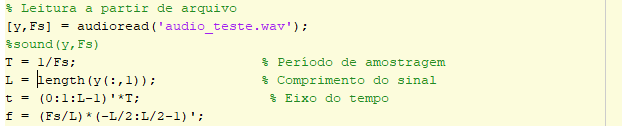
\includegraphics[width=0.7\textwidth]{graficos/code_audio.png}
        \end{figure} 
    	\begin{figure}[!htb]
        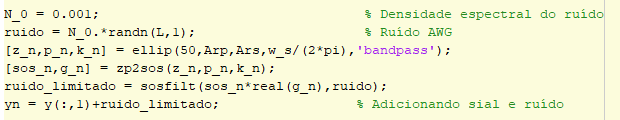
\includegraphics[width=0.7\textwidth]{graficos/code_ruido.png}
        \end{figure} 

\end{frame}

\begin{frame}{Áudio original}
    \begin{figure}[!htb]
        \centering
        \subfloat{
        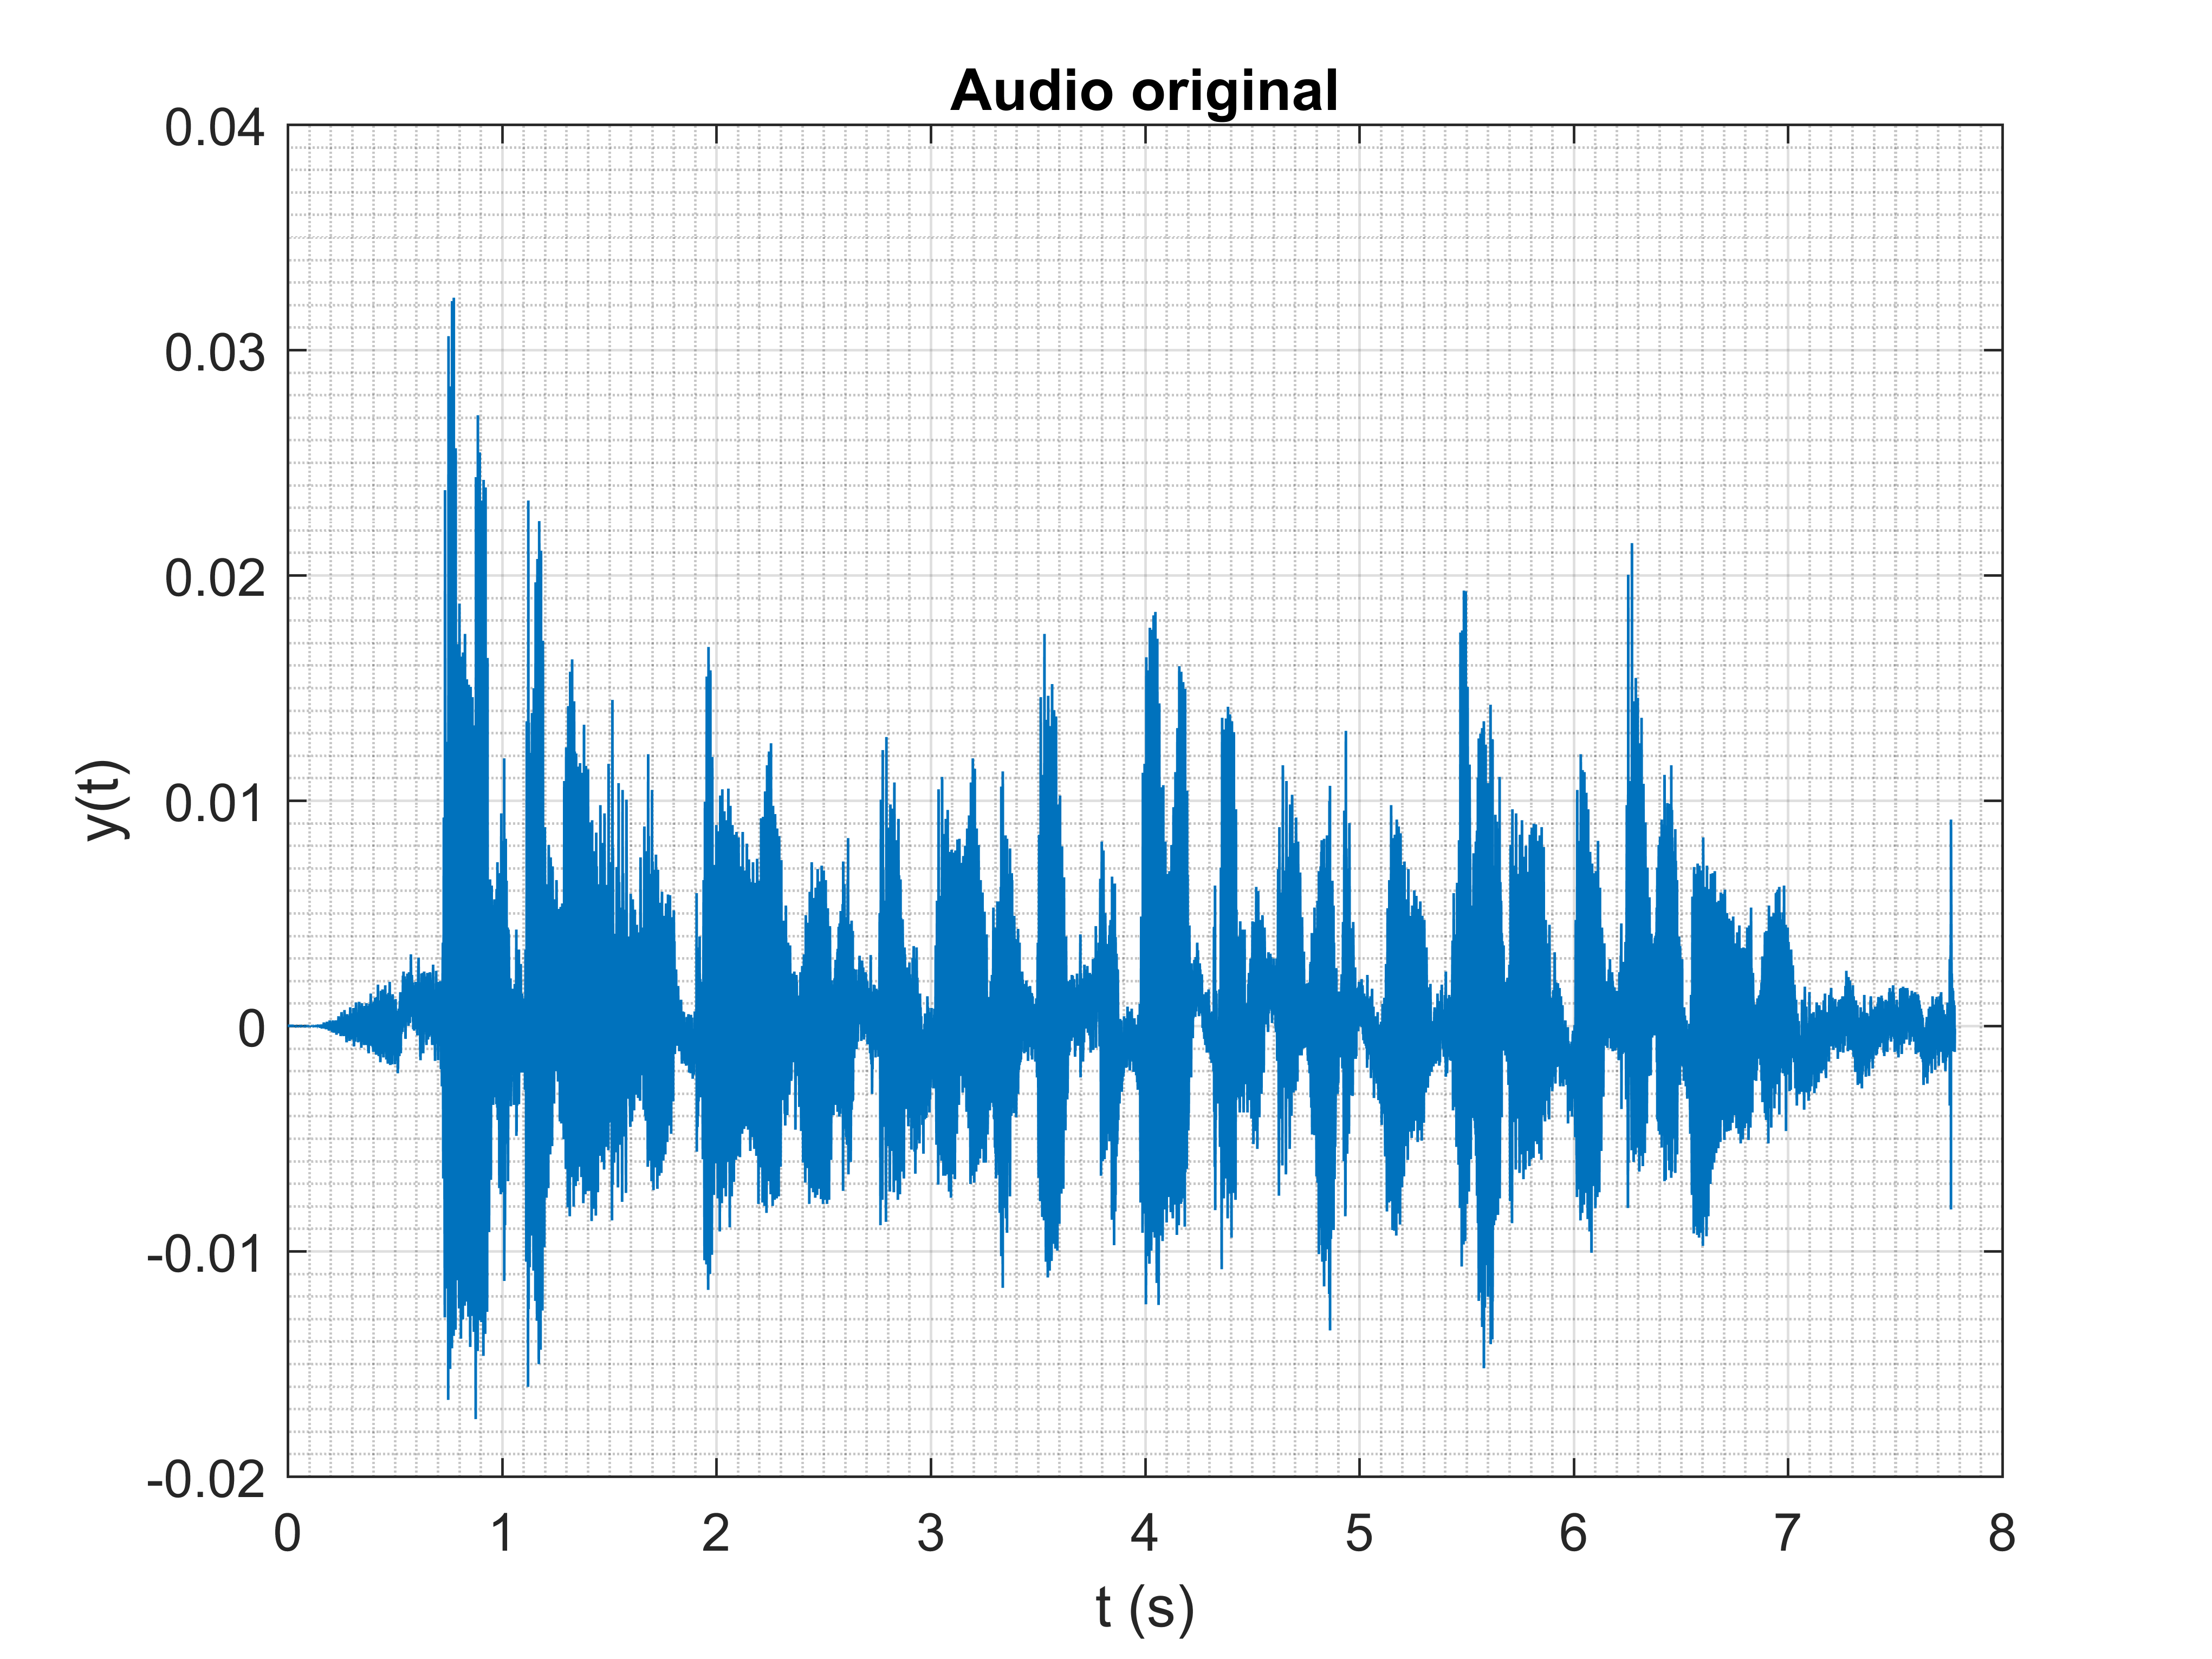
\includegraphics[scale=0.35]{graficos/audio_t.png}
        }
        \subfloat{
        \centering
        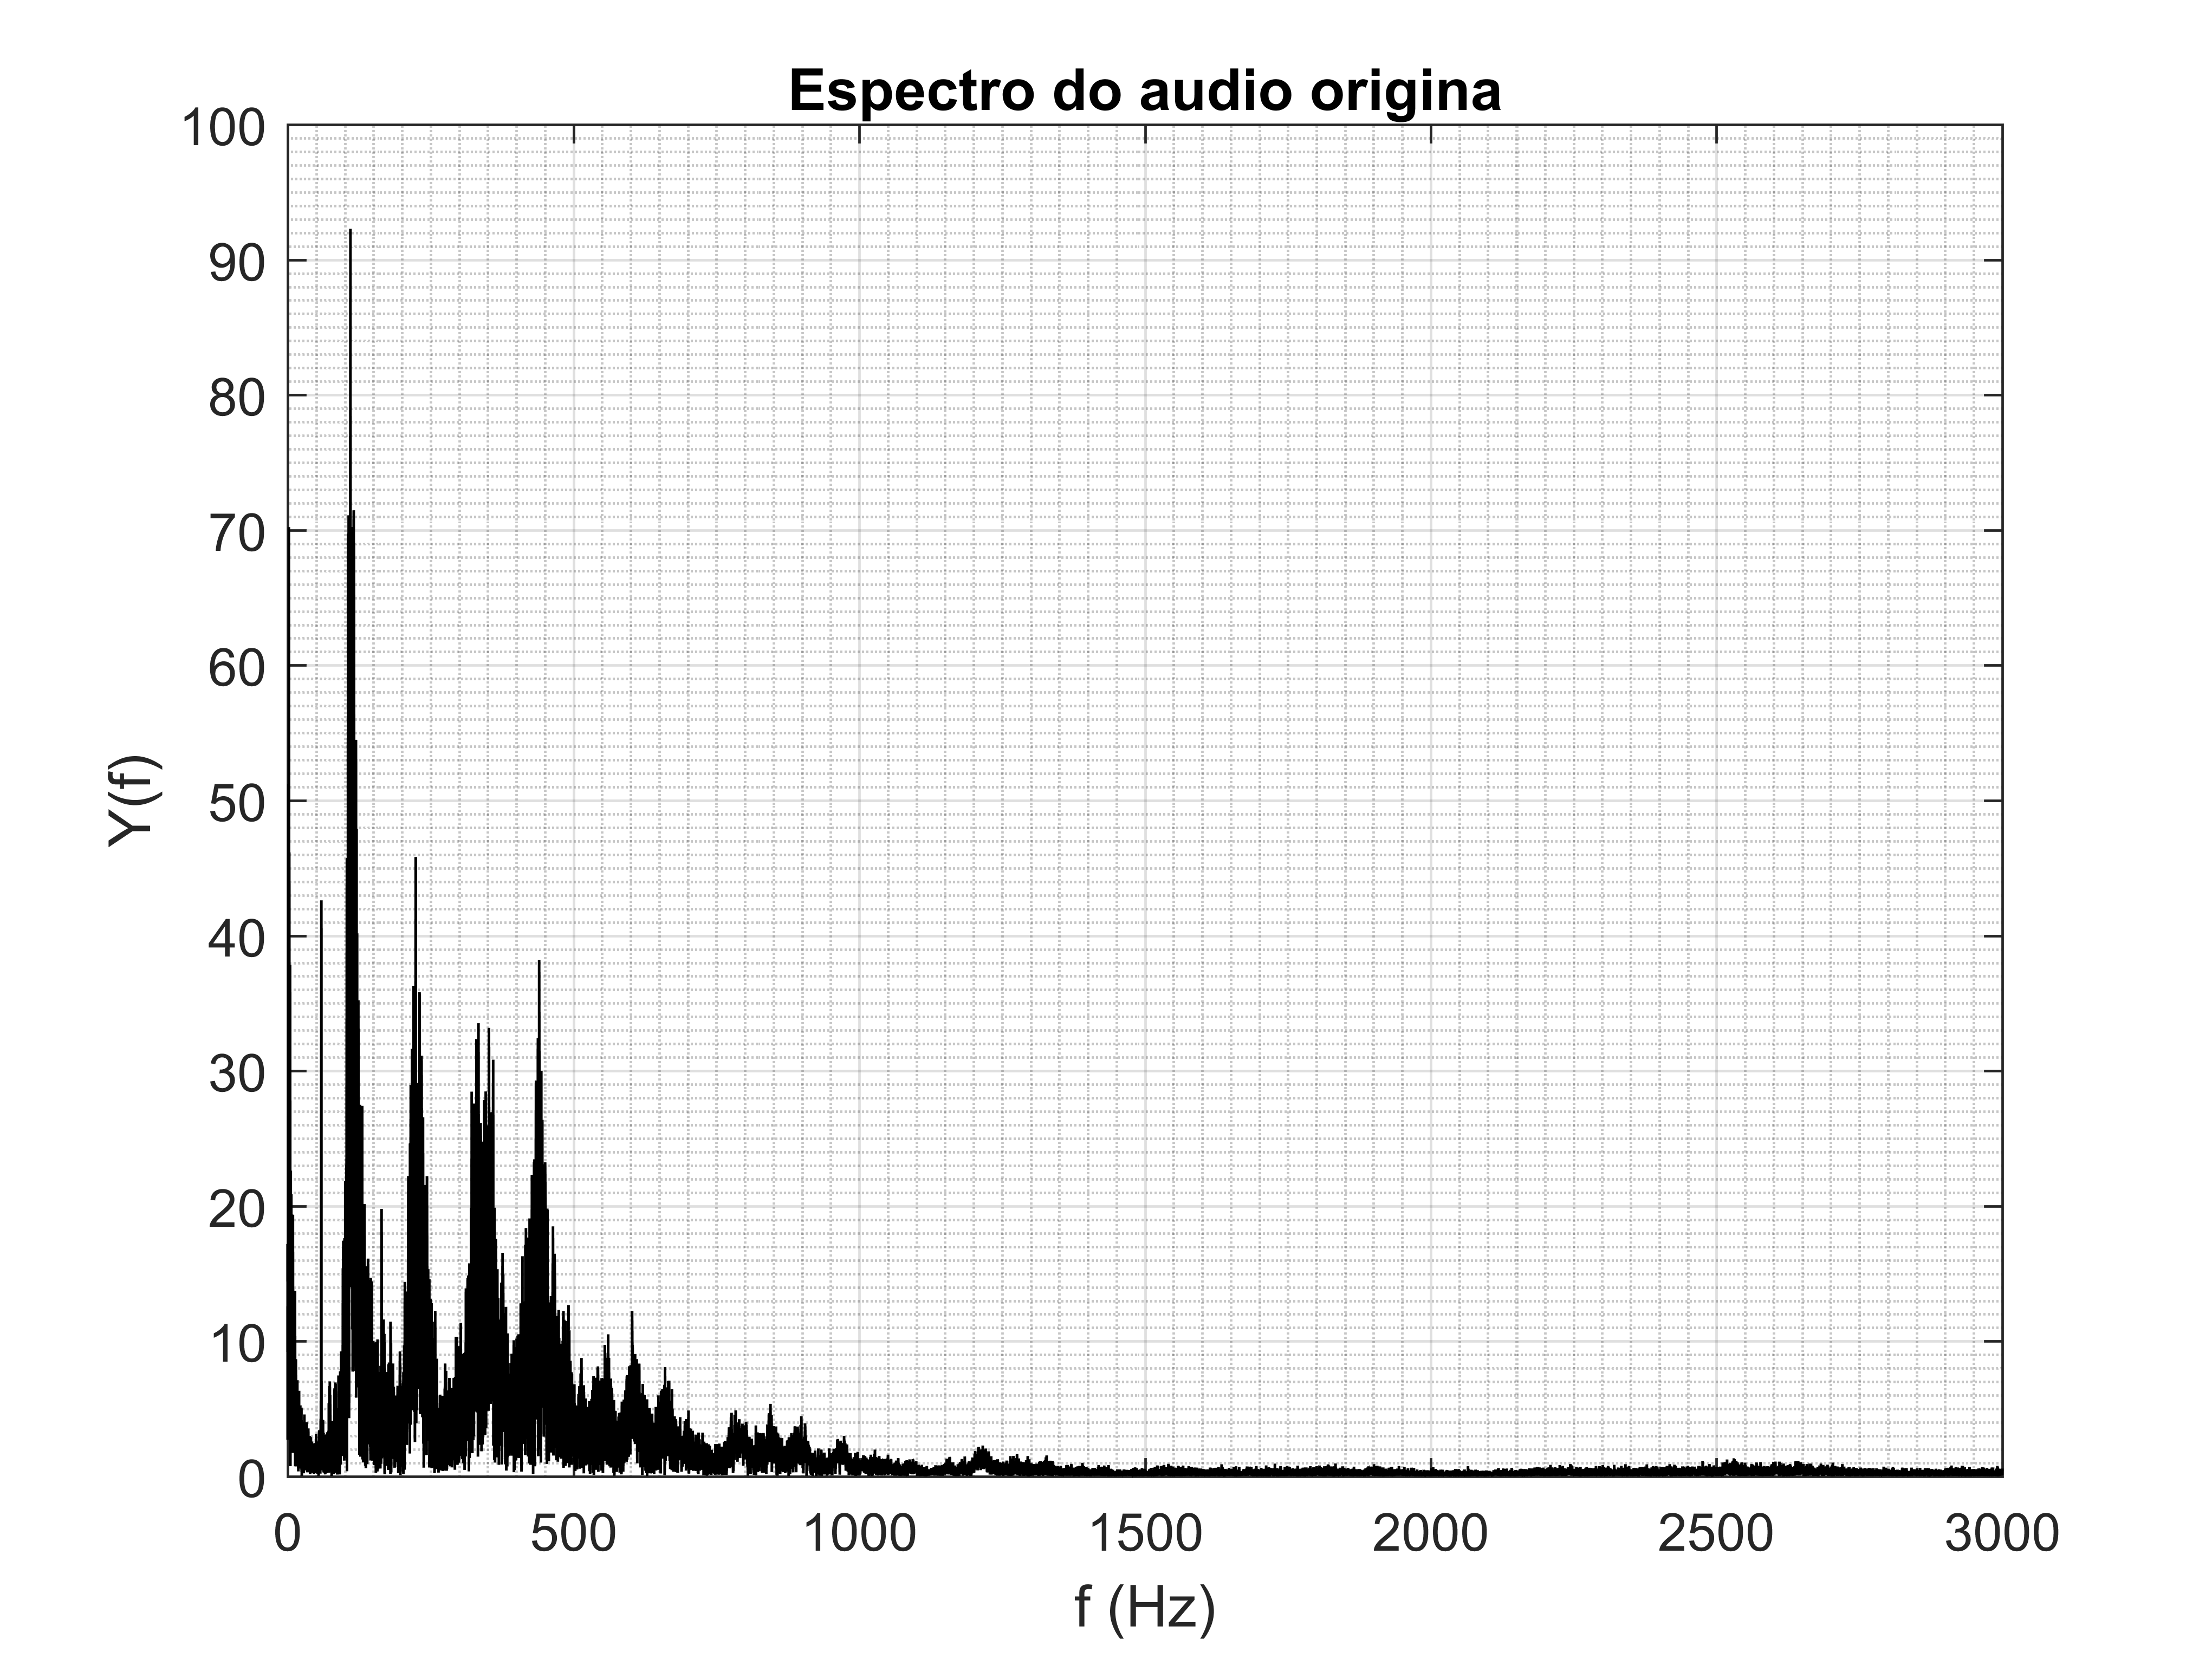
\includegraphics[scale=0.35]{graficos/audio_f.png}
        }
    \end{figure}   
\end{frame}

  

\begin{frame}{Ruído limitado em banda}
    \begin{figure}[!htb]
        \centering
        \subfloat{
        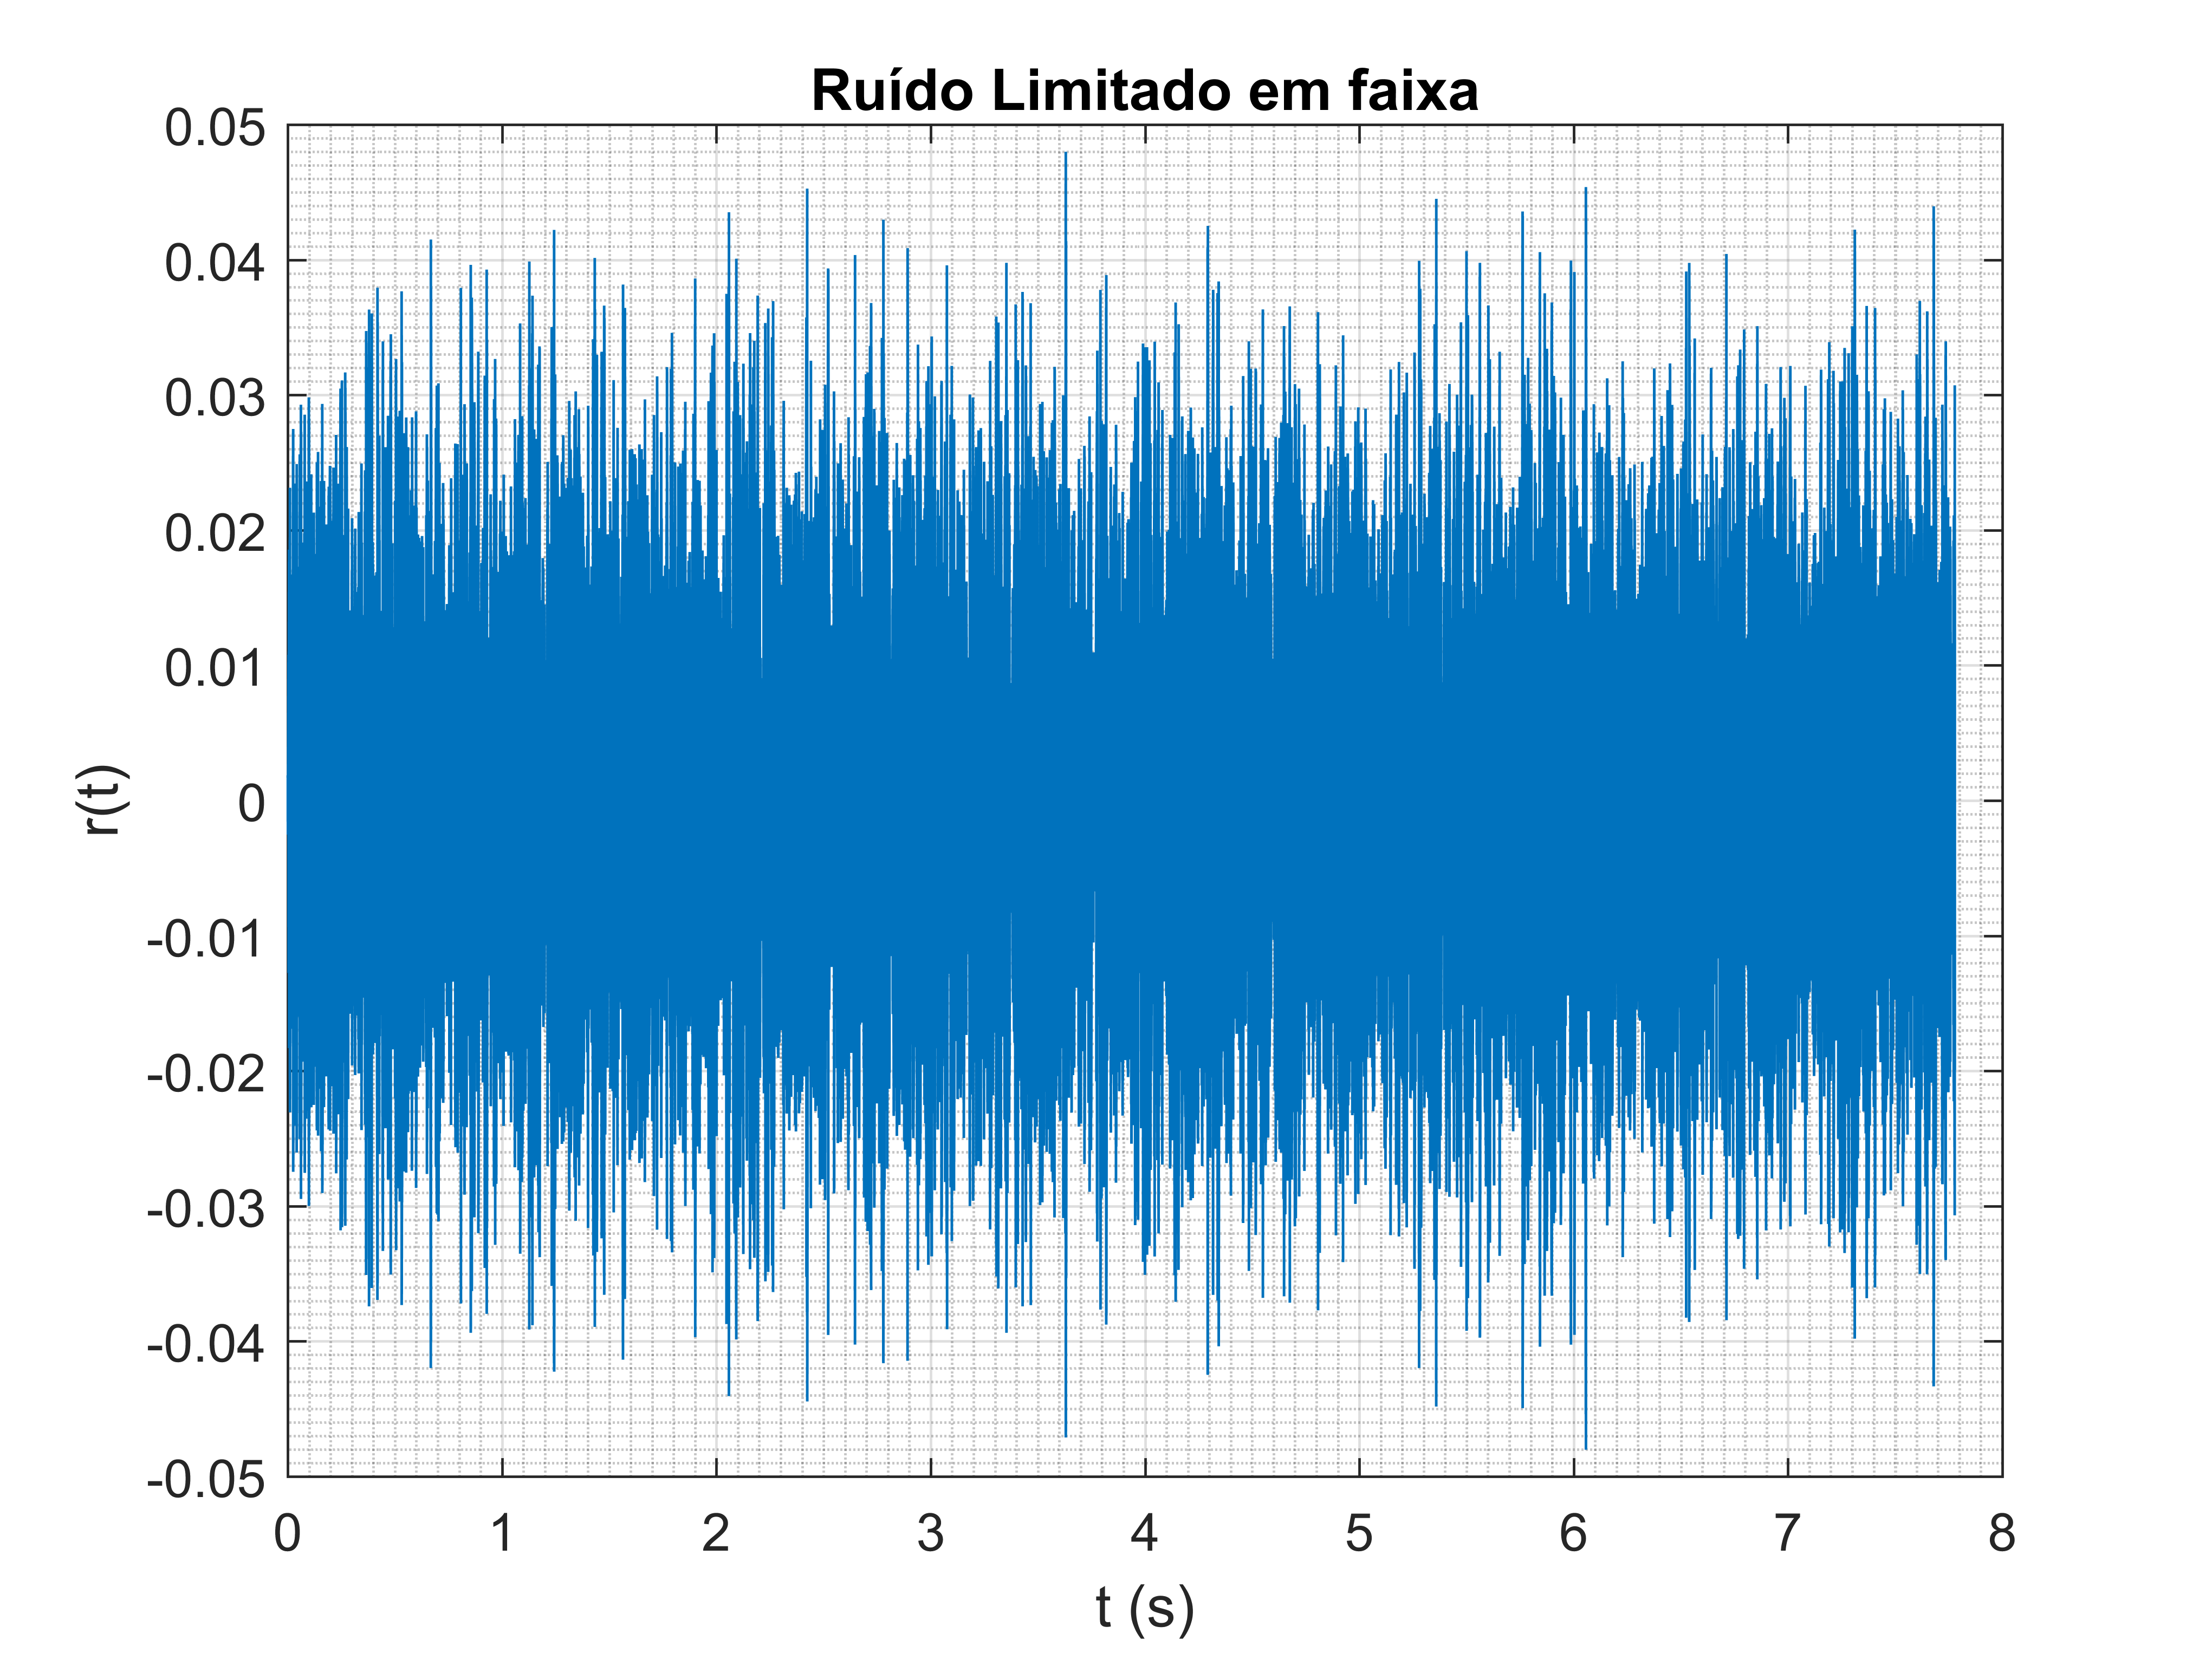
\includegraphics[scale=0.35]{graficos/ruido_limitado_t.png}
        }
        \subfloat{
        \centering
        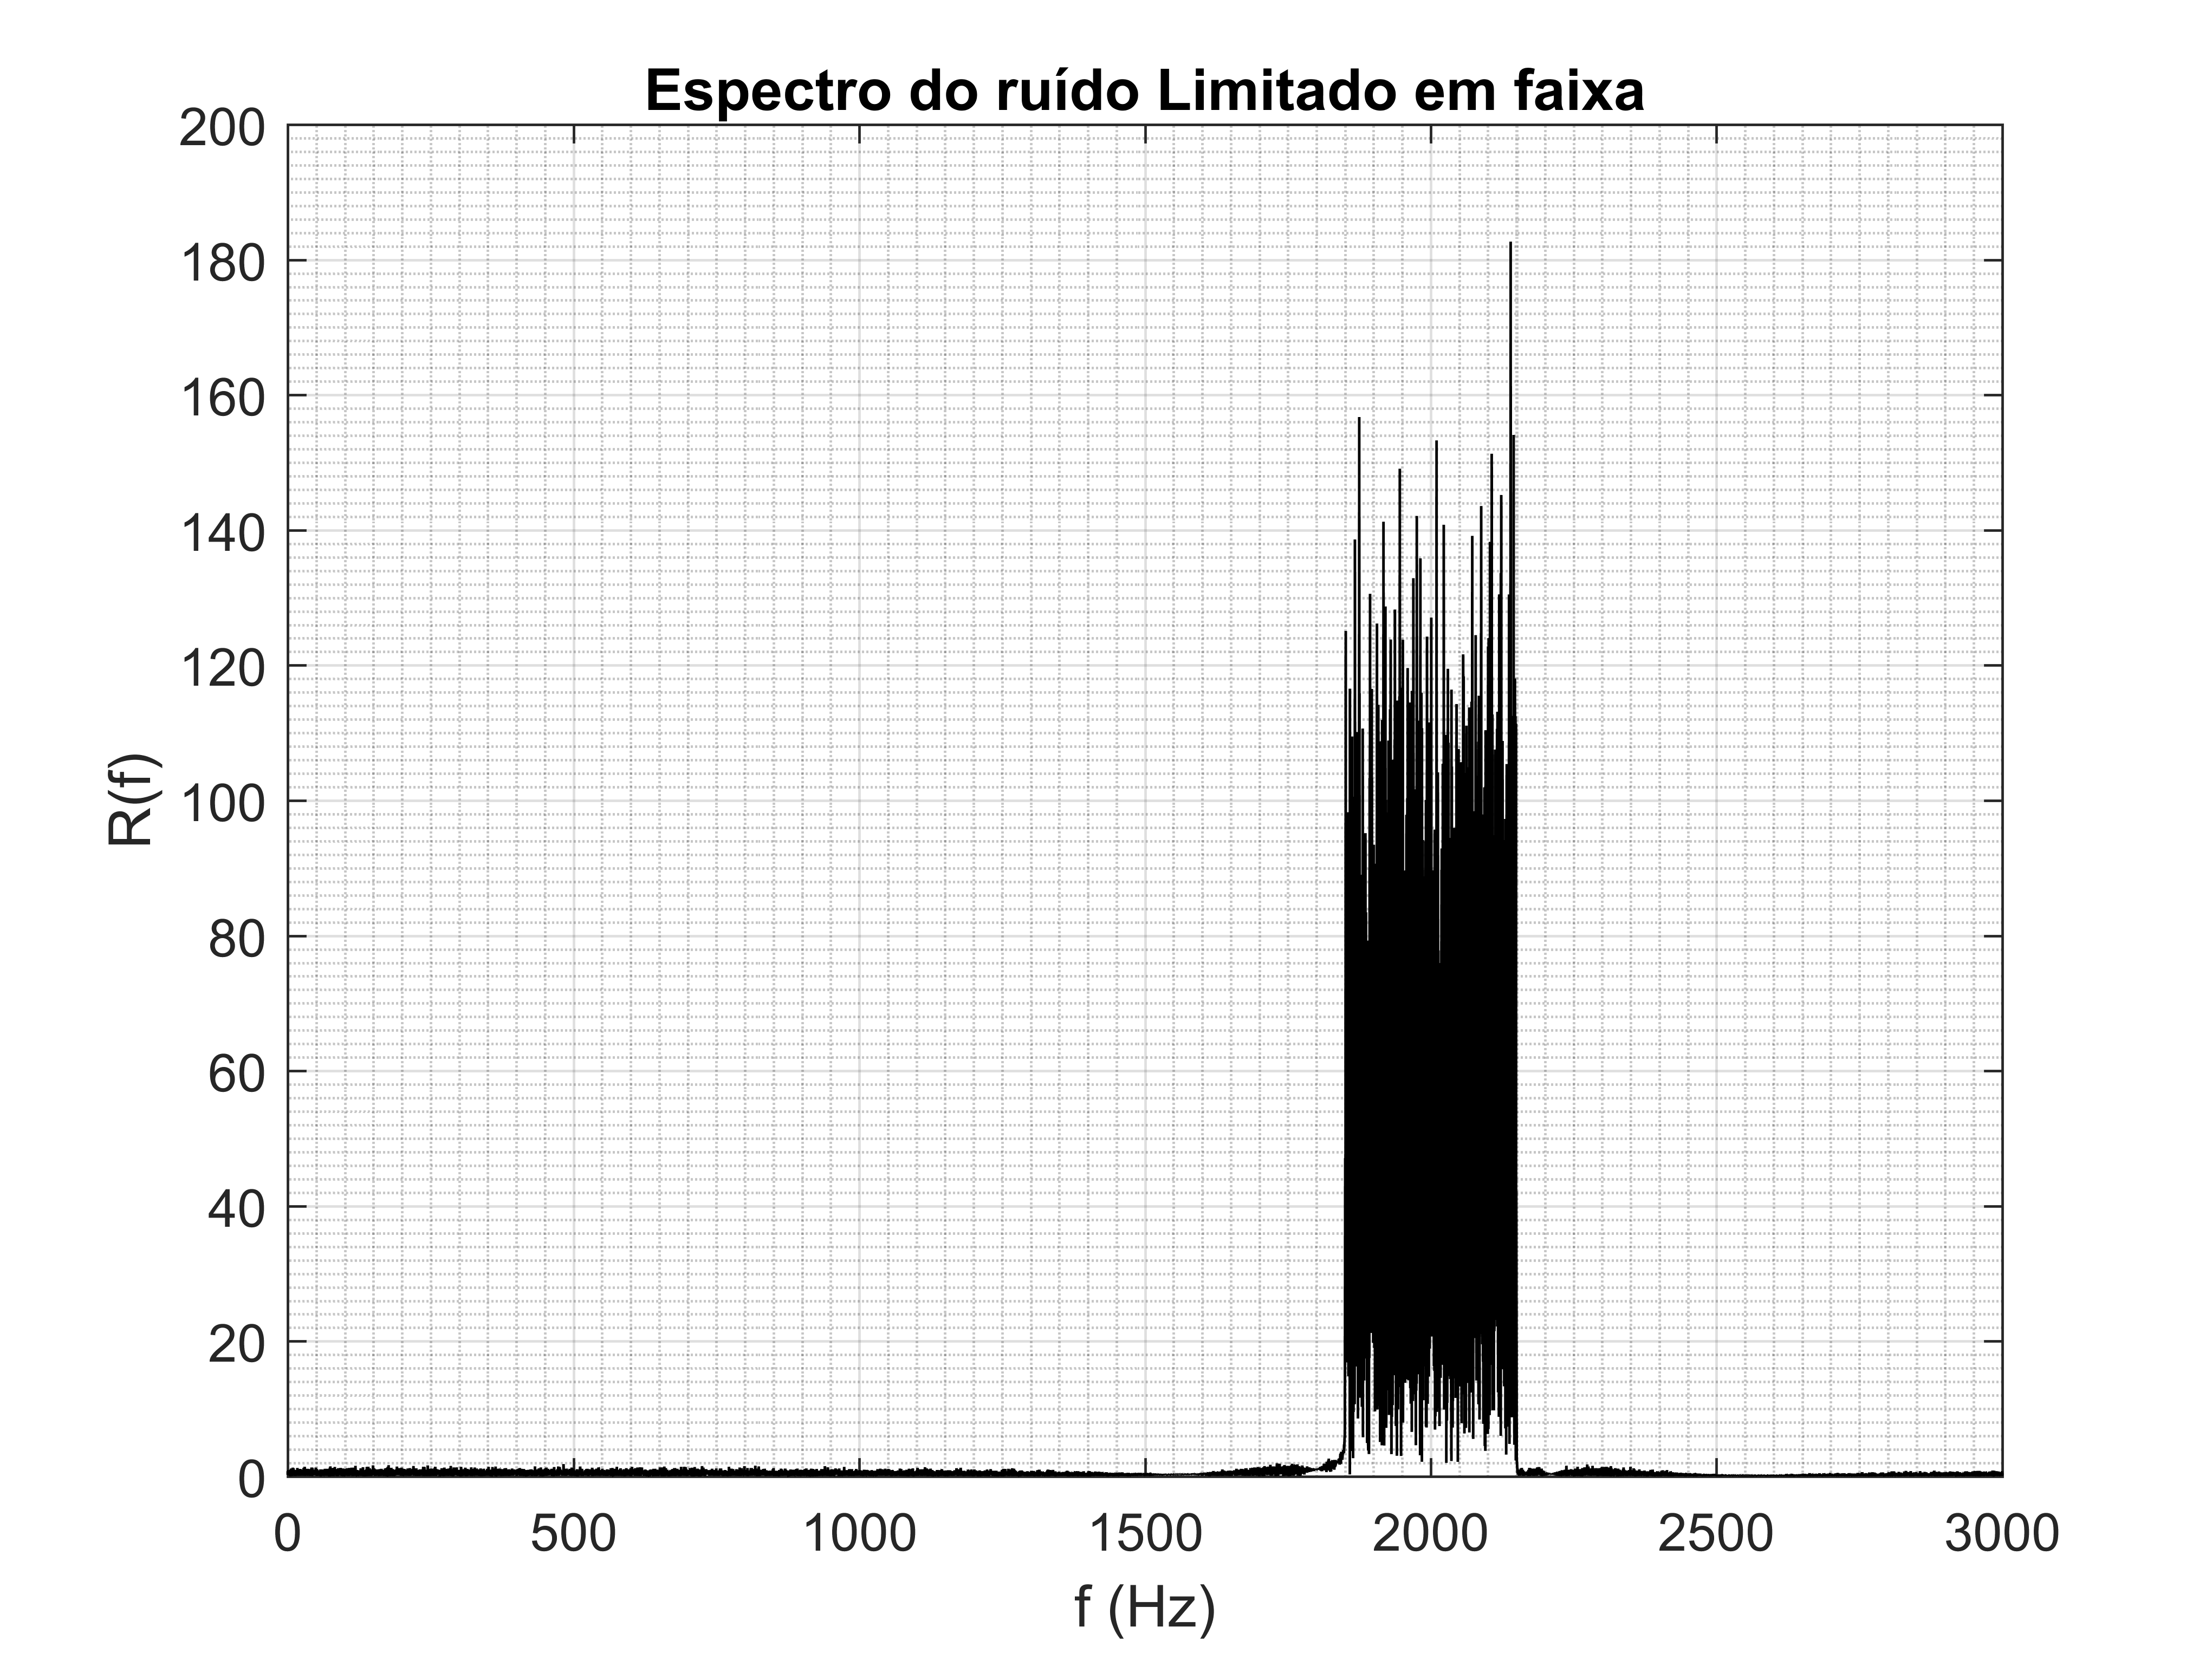
\includegraphics[scale=0.35]{graficos/ruido_limitado_f.png}
        }
    \end{figure}
    
\end{frame}

\begin{frame}{Áudio original corrompido pelo ruído}
    \begin{figure}[!htb]
        \centering
        \subfloat{
        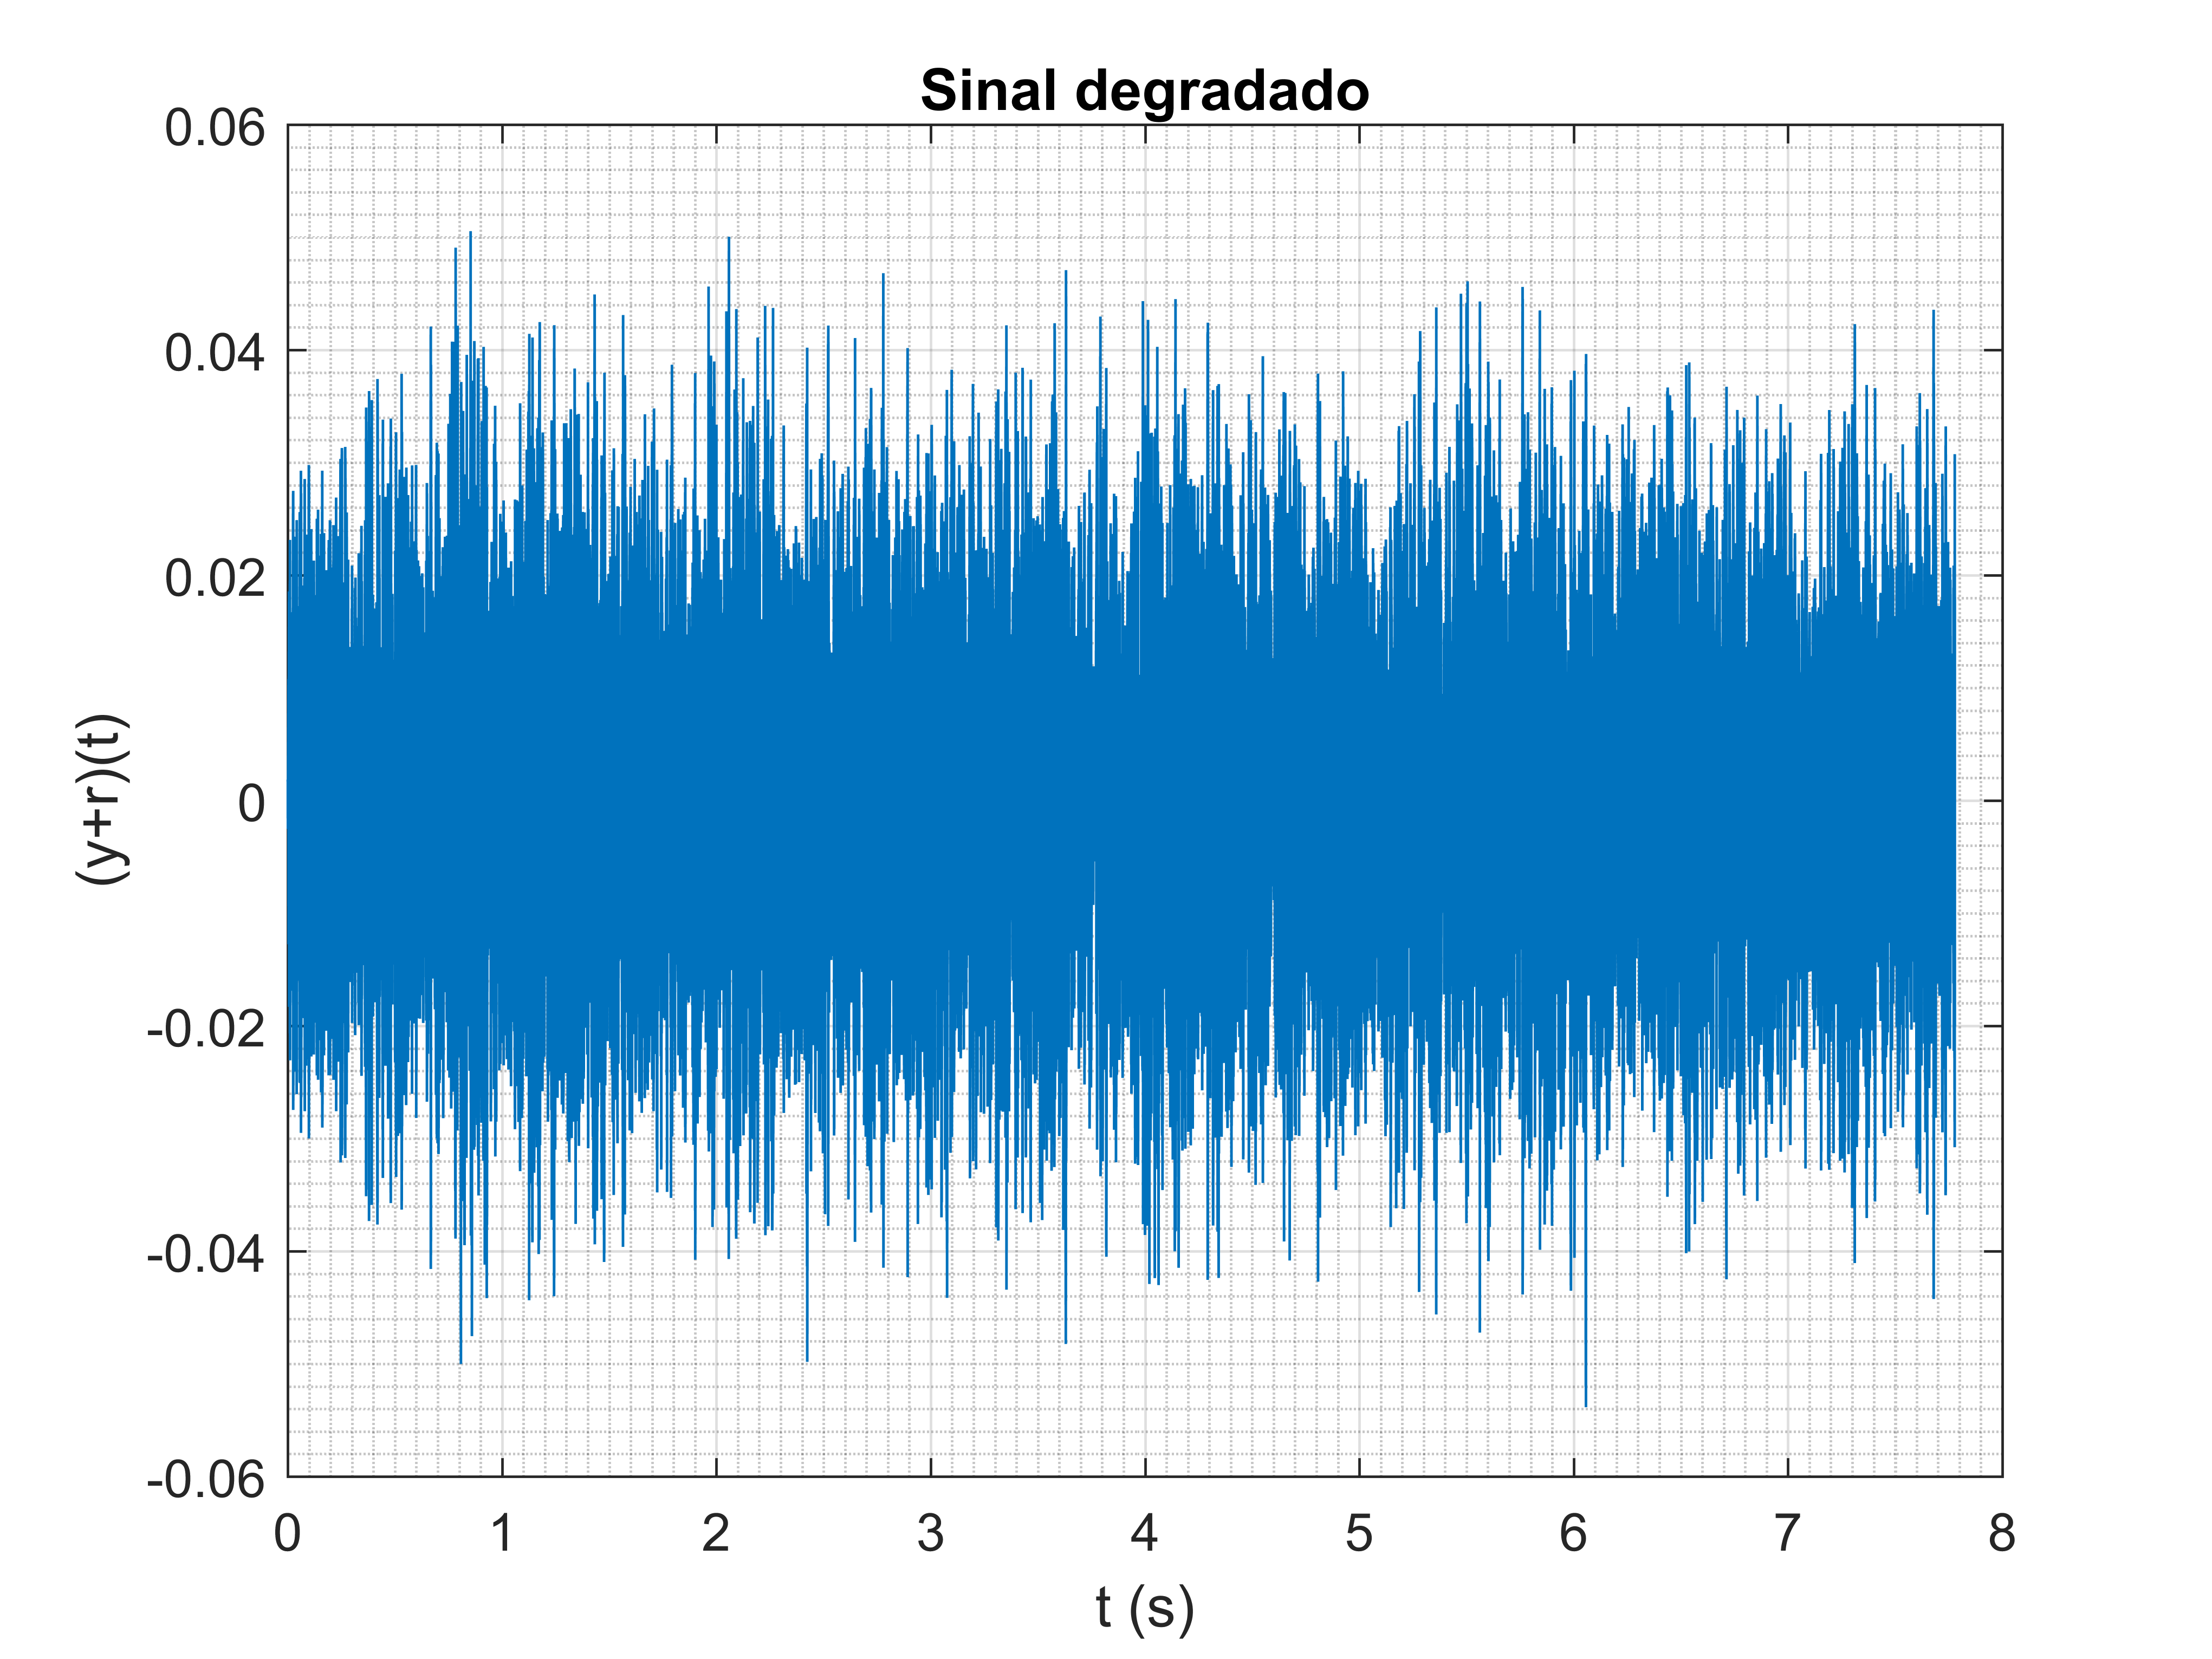
\includegraphics[scale=0.35]{graficos/sinal_ruido_t.png}
        }
        \subfloat{
        \centering
        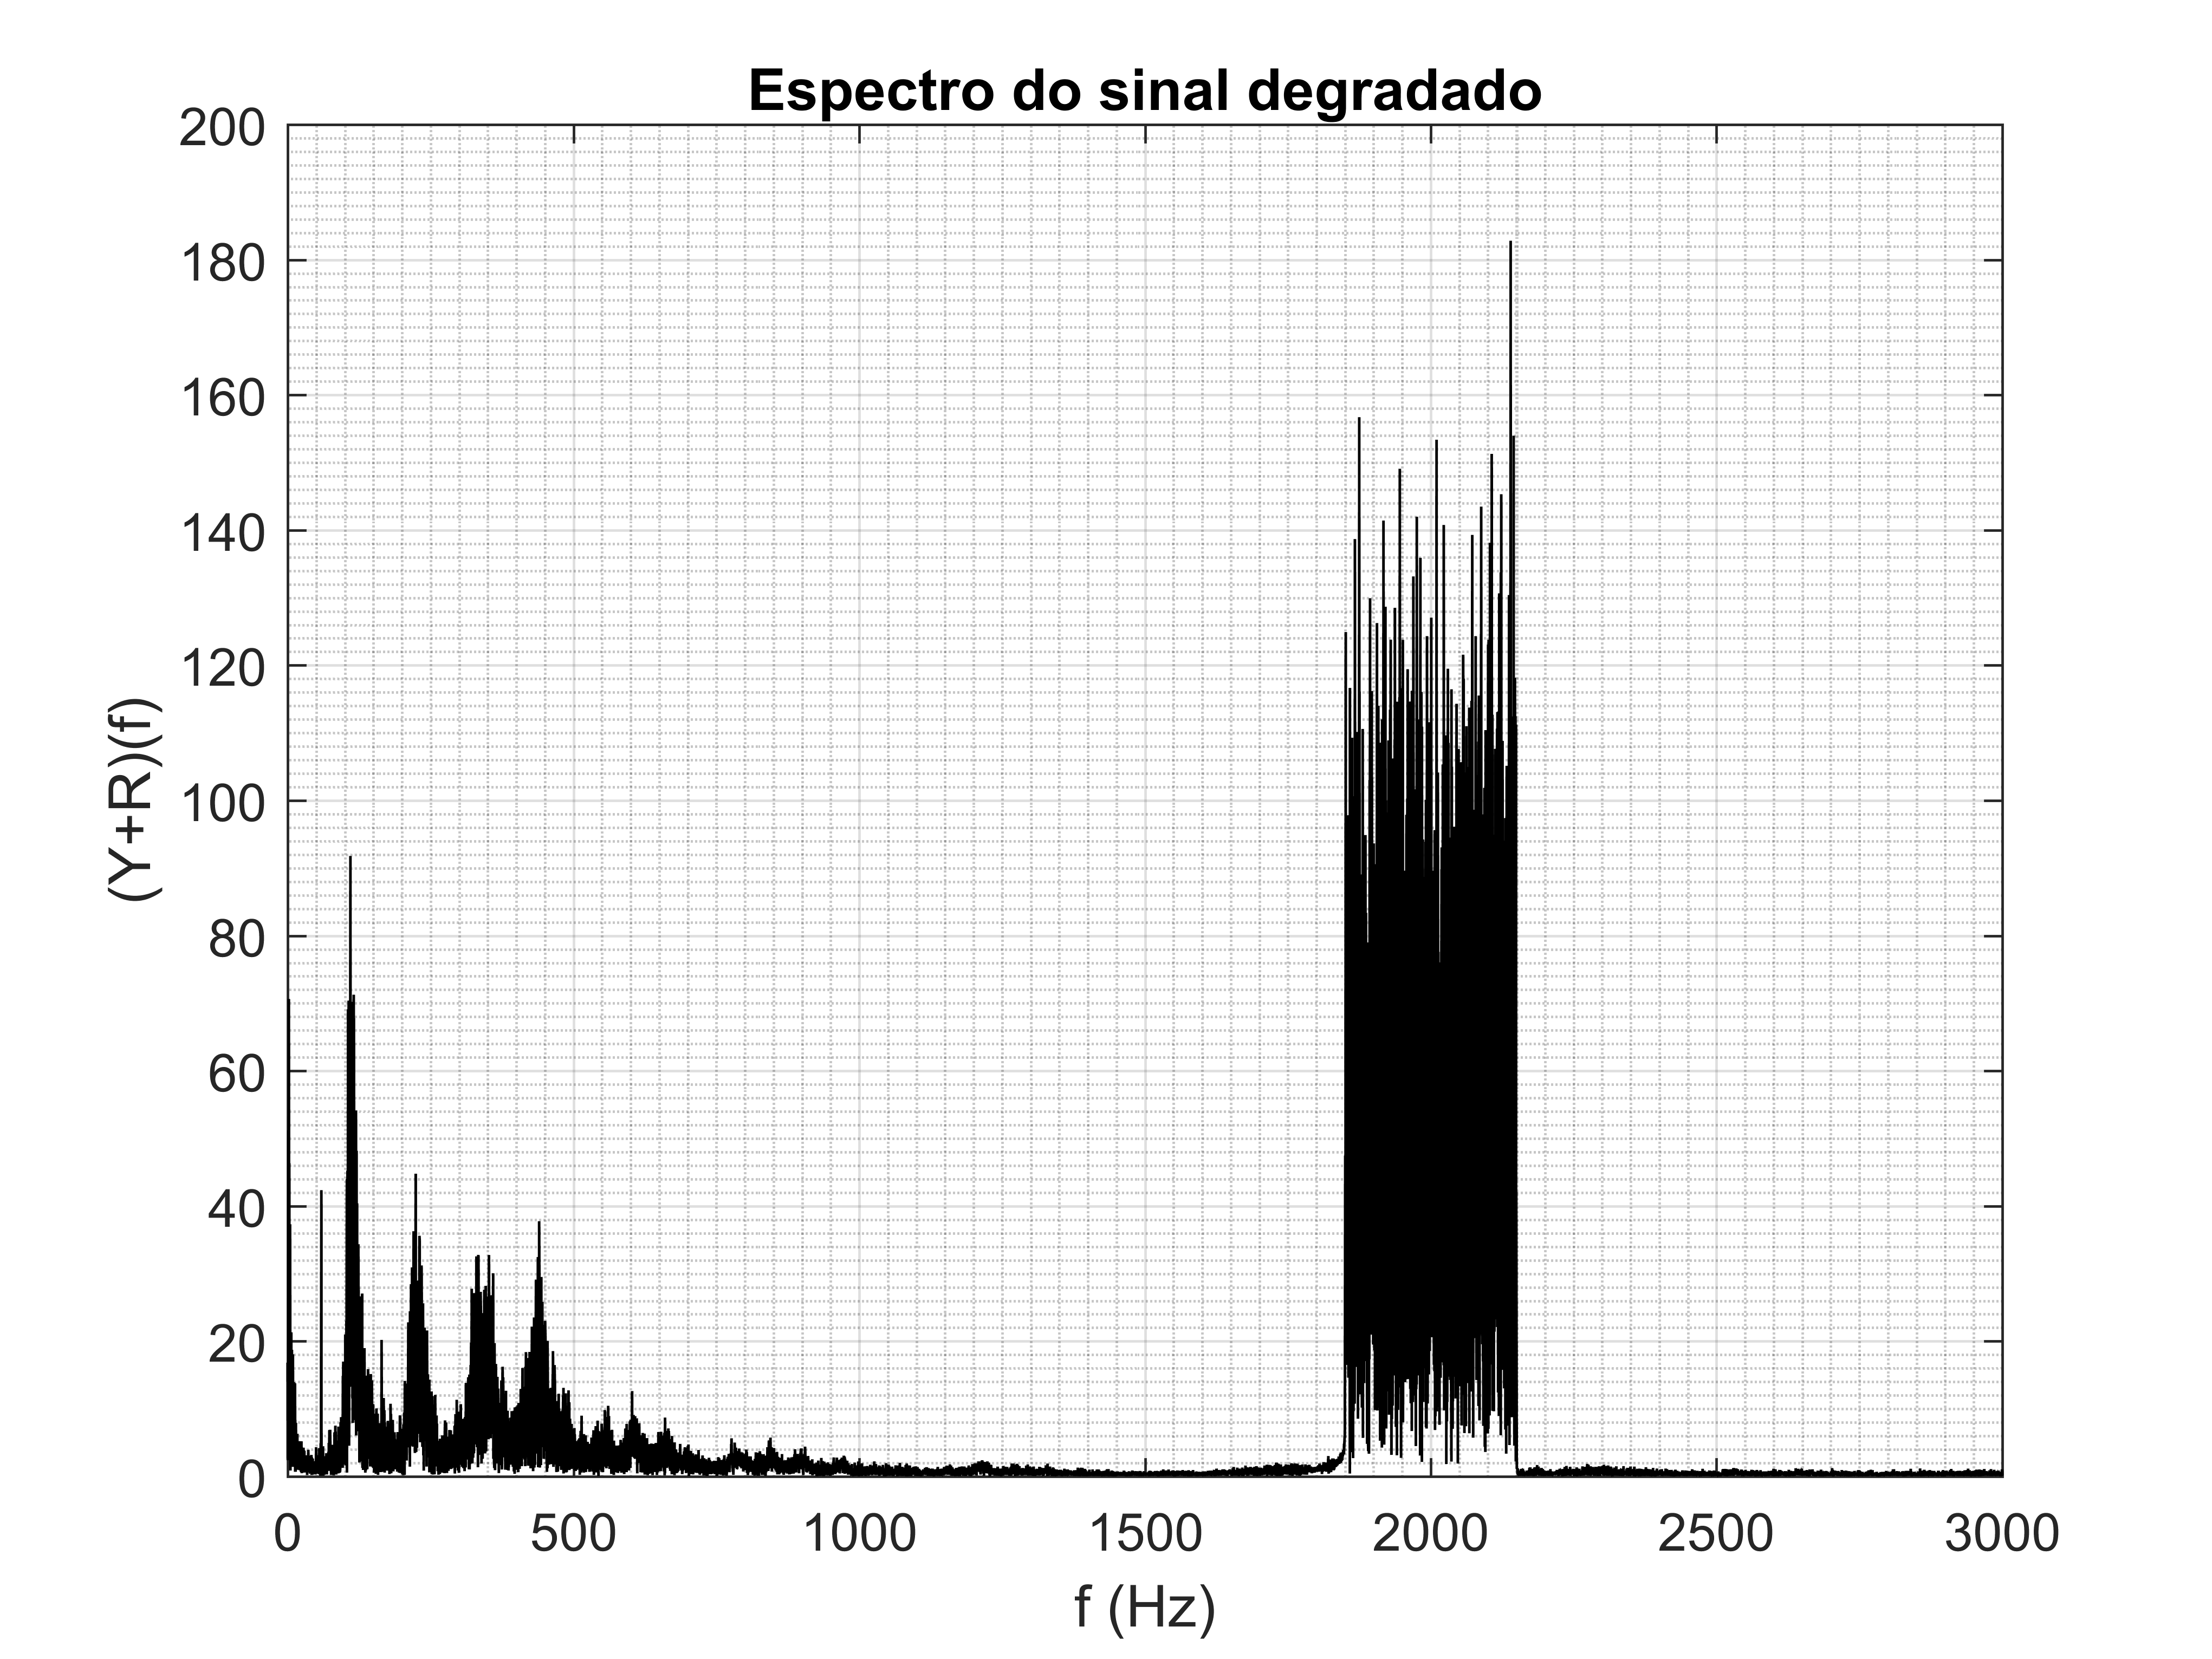
\includegraphics[scale=0.35]{graficos/sinal_ruido_f.png}
        }
    \end{figure}
\end{frame}


\begin{frame}{Especificações dos Filtros}
    \begin{itemize}
    \item Serão utilizadas 4 arquiteturas de filtros: Butterworth, Chebyshev I e II e Elíptico
        \item Os filtros serão passa-faixa com as especificações abaixo
            \begin{itemize}
                \item Limite da primeira faixa de passagem $\omega_{p1}$ = 2$\pi$1800
                \item Primeiro limite da faixa de rejeição $\omega_{s1}$ = 2$\pi$1850
                \item Segundo limite da faixa de rejeição $\omega_{p2}$ = 2$\pi$2150
                \item Limite da segunda faixa de passagem $\omega_{s2}$ = 2$\pi$2200
                \item Variação máxima de ganho nas faixas de passagem e transição $\epsilon$ = $\delta$ = 0.01 
            \end{itemize}
        
        \item Projetados usando técnicas de filtros analógicos
        
        \item Posteriormente discretizados usando transformação bilinear  
        
    \end{itemize}
\end{frame}

\begin{frame}{Especificações dos Filtros}
    \begin{figure}[!htb]
        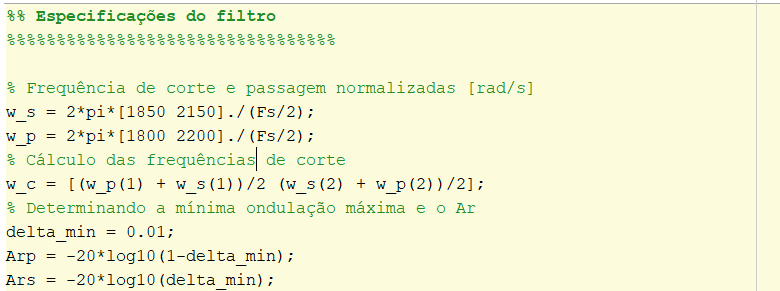
\includegraphics[width=0.9\textwidth]{graficos/especificacoes.png}
        \end{figure} 
\end{frame}

\begin{frame}{Gabarito do Filtro}
    	\begin{figure}[!htb]
        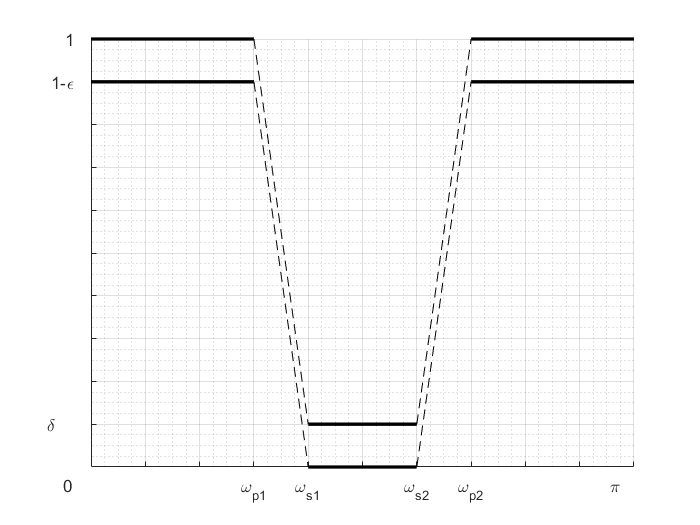
\includegraphics[width=0.7\textwidth]{graficos/gabarito.png}
        \end{figure} 
\end{frame}

\begin{frame}{Tentativa 1 de cálculo de H(s)=N(s)/D(s)}
\begin{itemize}
    \item A ordem do primeiro filtro (Butterworth) foi de 50
    \item Não foi possível representar adequadamente os polinômios
    
\end{itemize}
    \begin{figure}[!htb]
    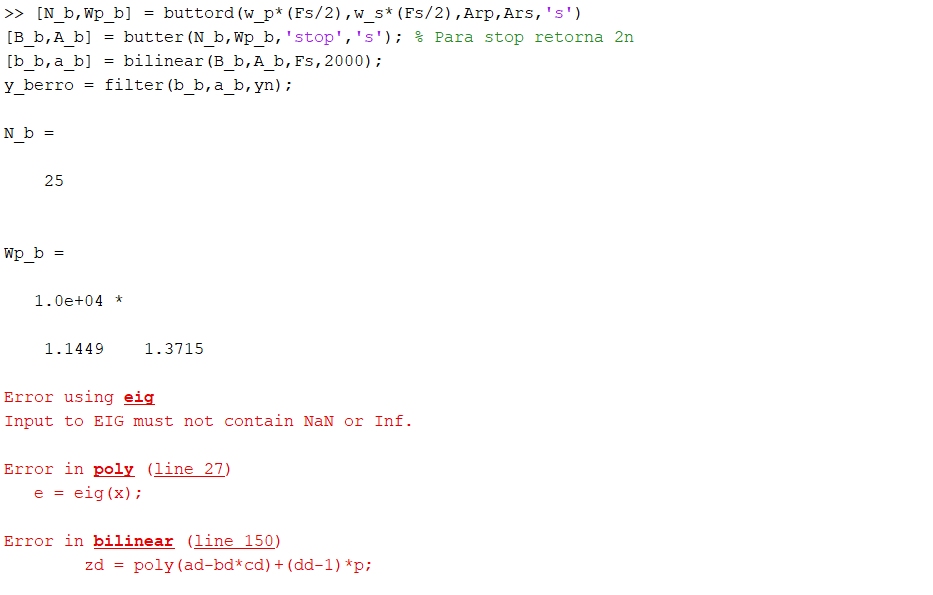
\includegraphics[width=0.6\textwidth]{graficos/num_dem_try_1_erro.png}
    \end{figure}
    
\end{frame}

\begin{frame}{Tentativa 1 de cálculo de H(s)=N(s)/D(s)}
        \begin{figure}[!htb]
        \centering
        \subfloat{
        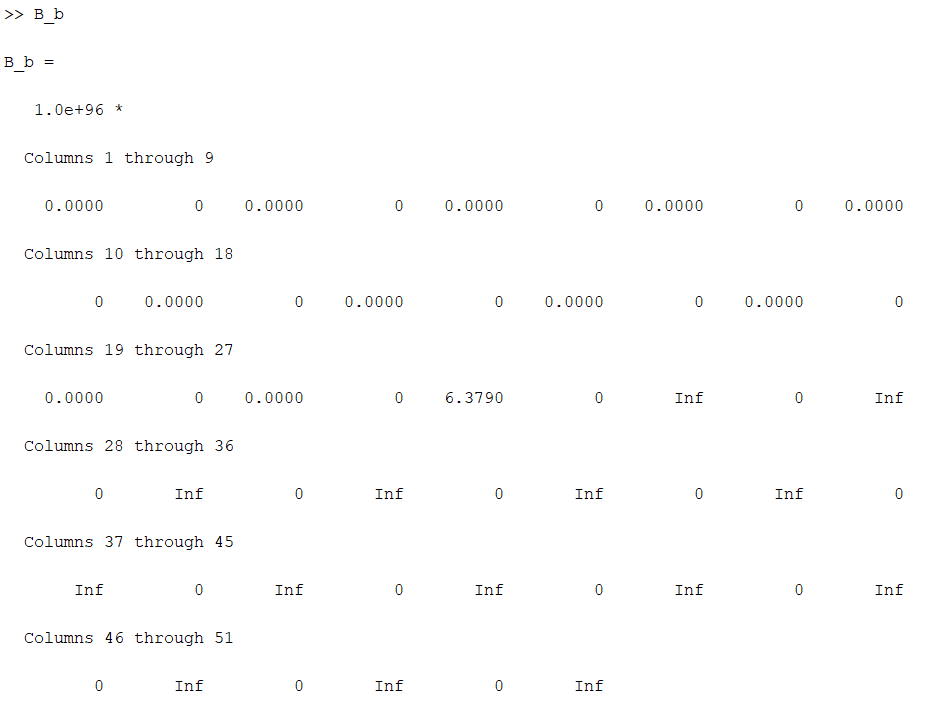
\includegraphics[scale=0.28]{graficos/num_dem_try_1_zeros.png}
        }
        \subfloat{
        \centering
        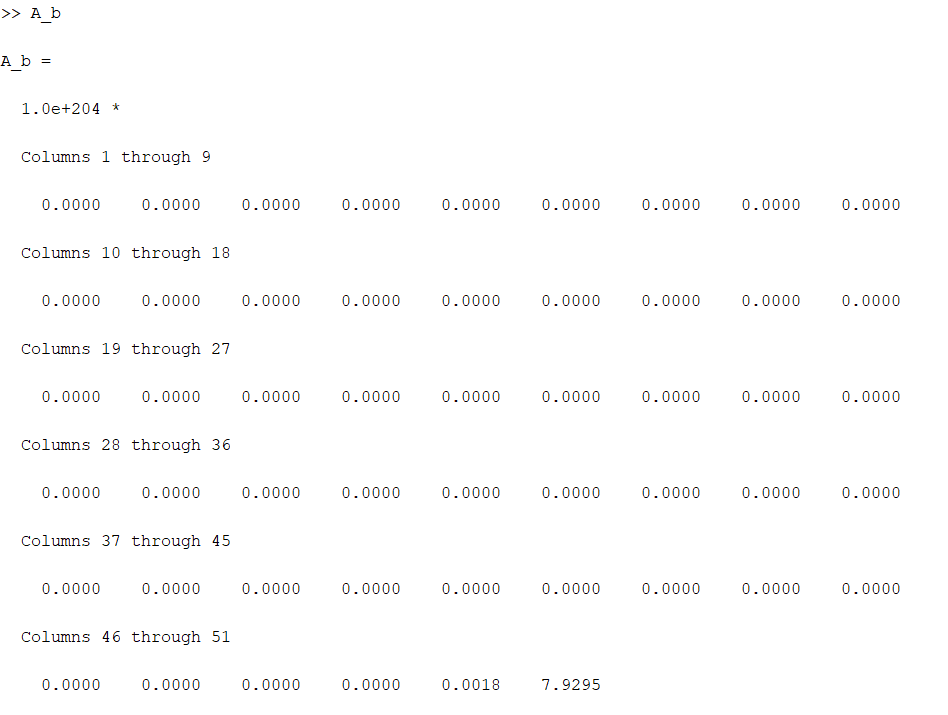
\includegraphics[scale=0.28]{graficos/num_dem_try_1_polos.png}
        }
    \end{figure}
\end{frame}

\begin{frame}{Tentativa 2 de cálculo de H(s)=N(s)/D(s)}
    \begin{itemize}
        \item Numa segunda tentativa foram calculados pólos e zeros fatorados
        \item Os pólos/zeros obtidos estavam no SPE (estáveis/fase mínima)
        \item Converteu-se estes pólos/zeros num polinômio D(s) e outro N(s)
        \item Novamente o polinômio obtido não representava adequadamente o filtro desejado
        \item Vários dos pólos/zeros do novo polinômio passaram a se localizar no SPD (instáveis/fase não-mínima)
    \end{itemize}
\end{frame}

\begin{frame}{Tentativa 2 de cálculo de H(s)=N(s)/D(s)}
    O diagrama de pólos e zeros mostra onde estavam os pólos e zeros originais (vermelhos) e onde passaram a ficar após serem tranformados em um polinômio de ordem alta (pretos)
    \begin{figure}[!htb]
    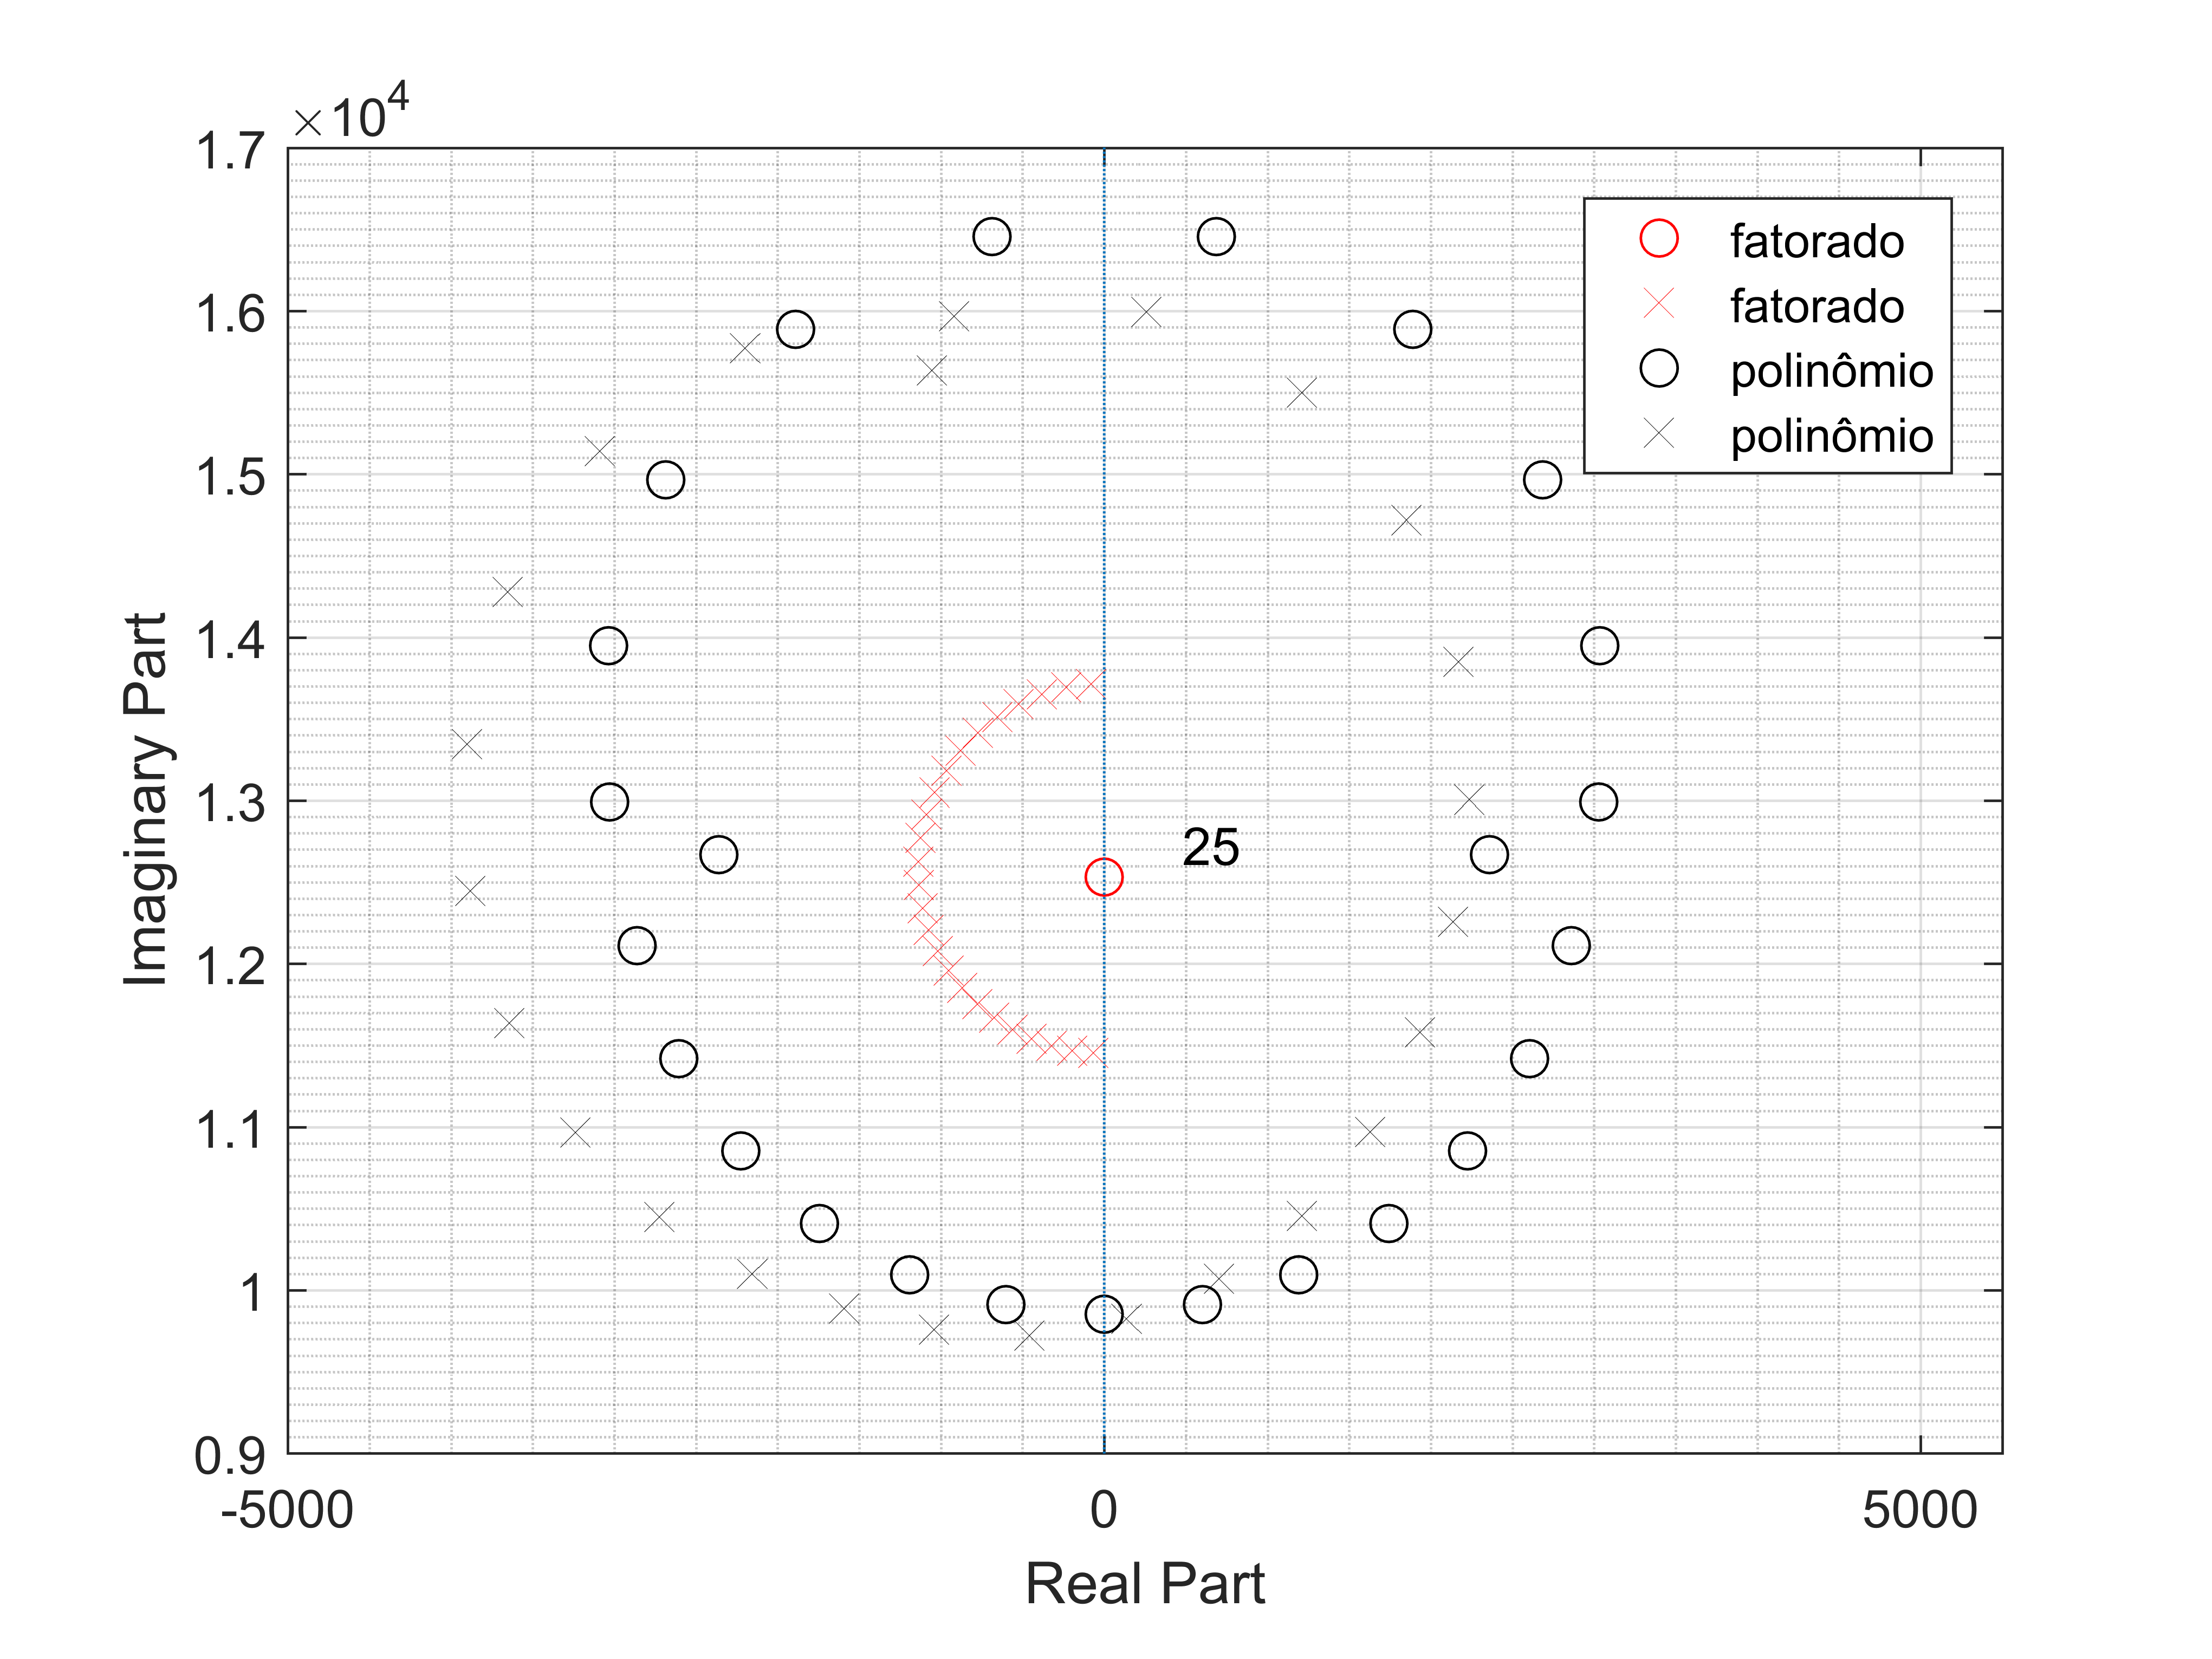
\includegraphics[width=0.6\textwidth]{graficos/z_plane_zpk_tf.PNG}
    \end{figure} 
    
\end{frame}

\begin{frame}{Tentativa 2 de cálculo de H(s)=N(s)/D(s)}
    Apenas para fins de análise o filtro instável foi discretizado e usado na filtragem do sinal. Como esperado, houve overflow com poucos milisegundos
        \begin{figure}[!htb]
    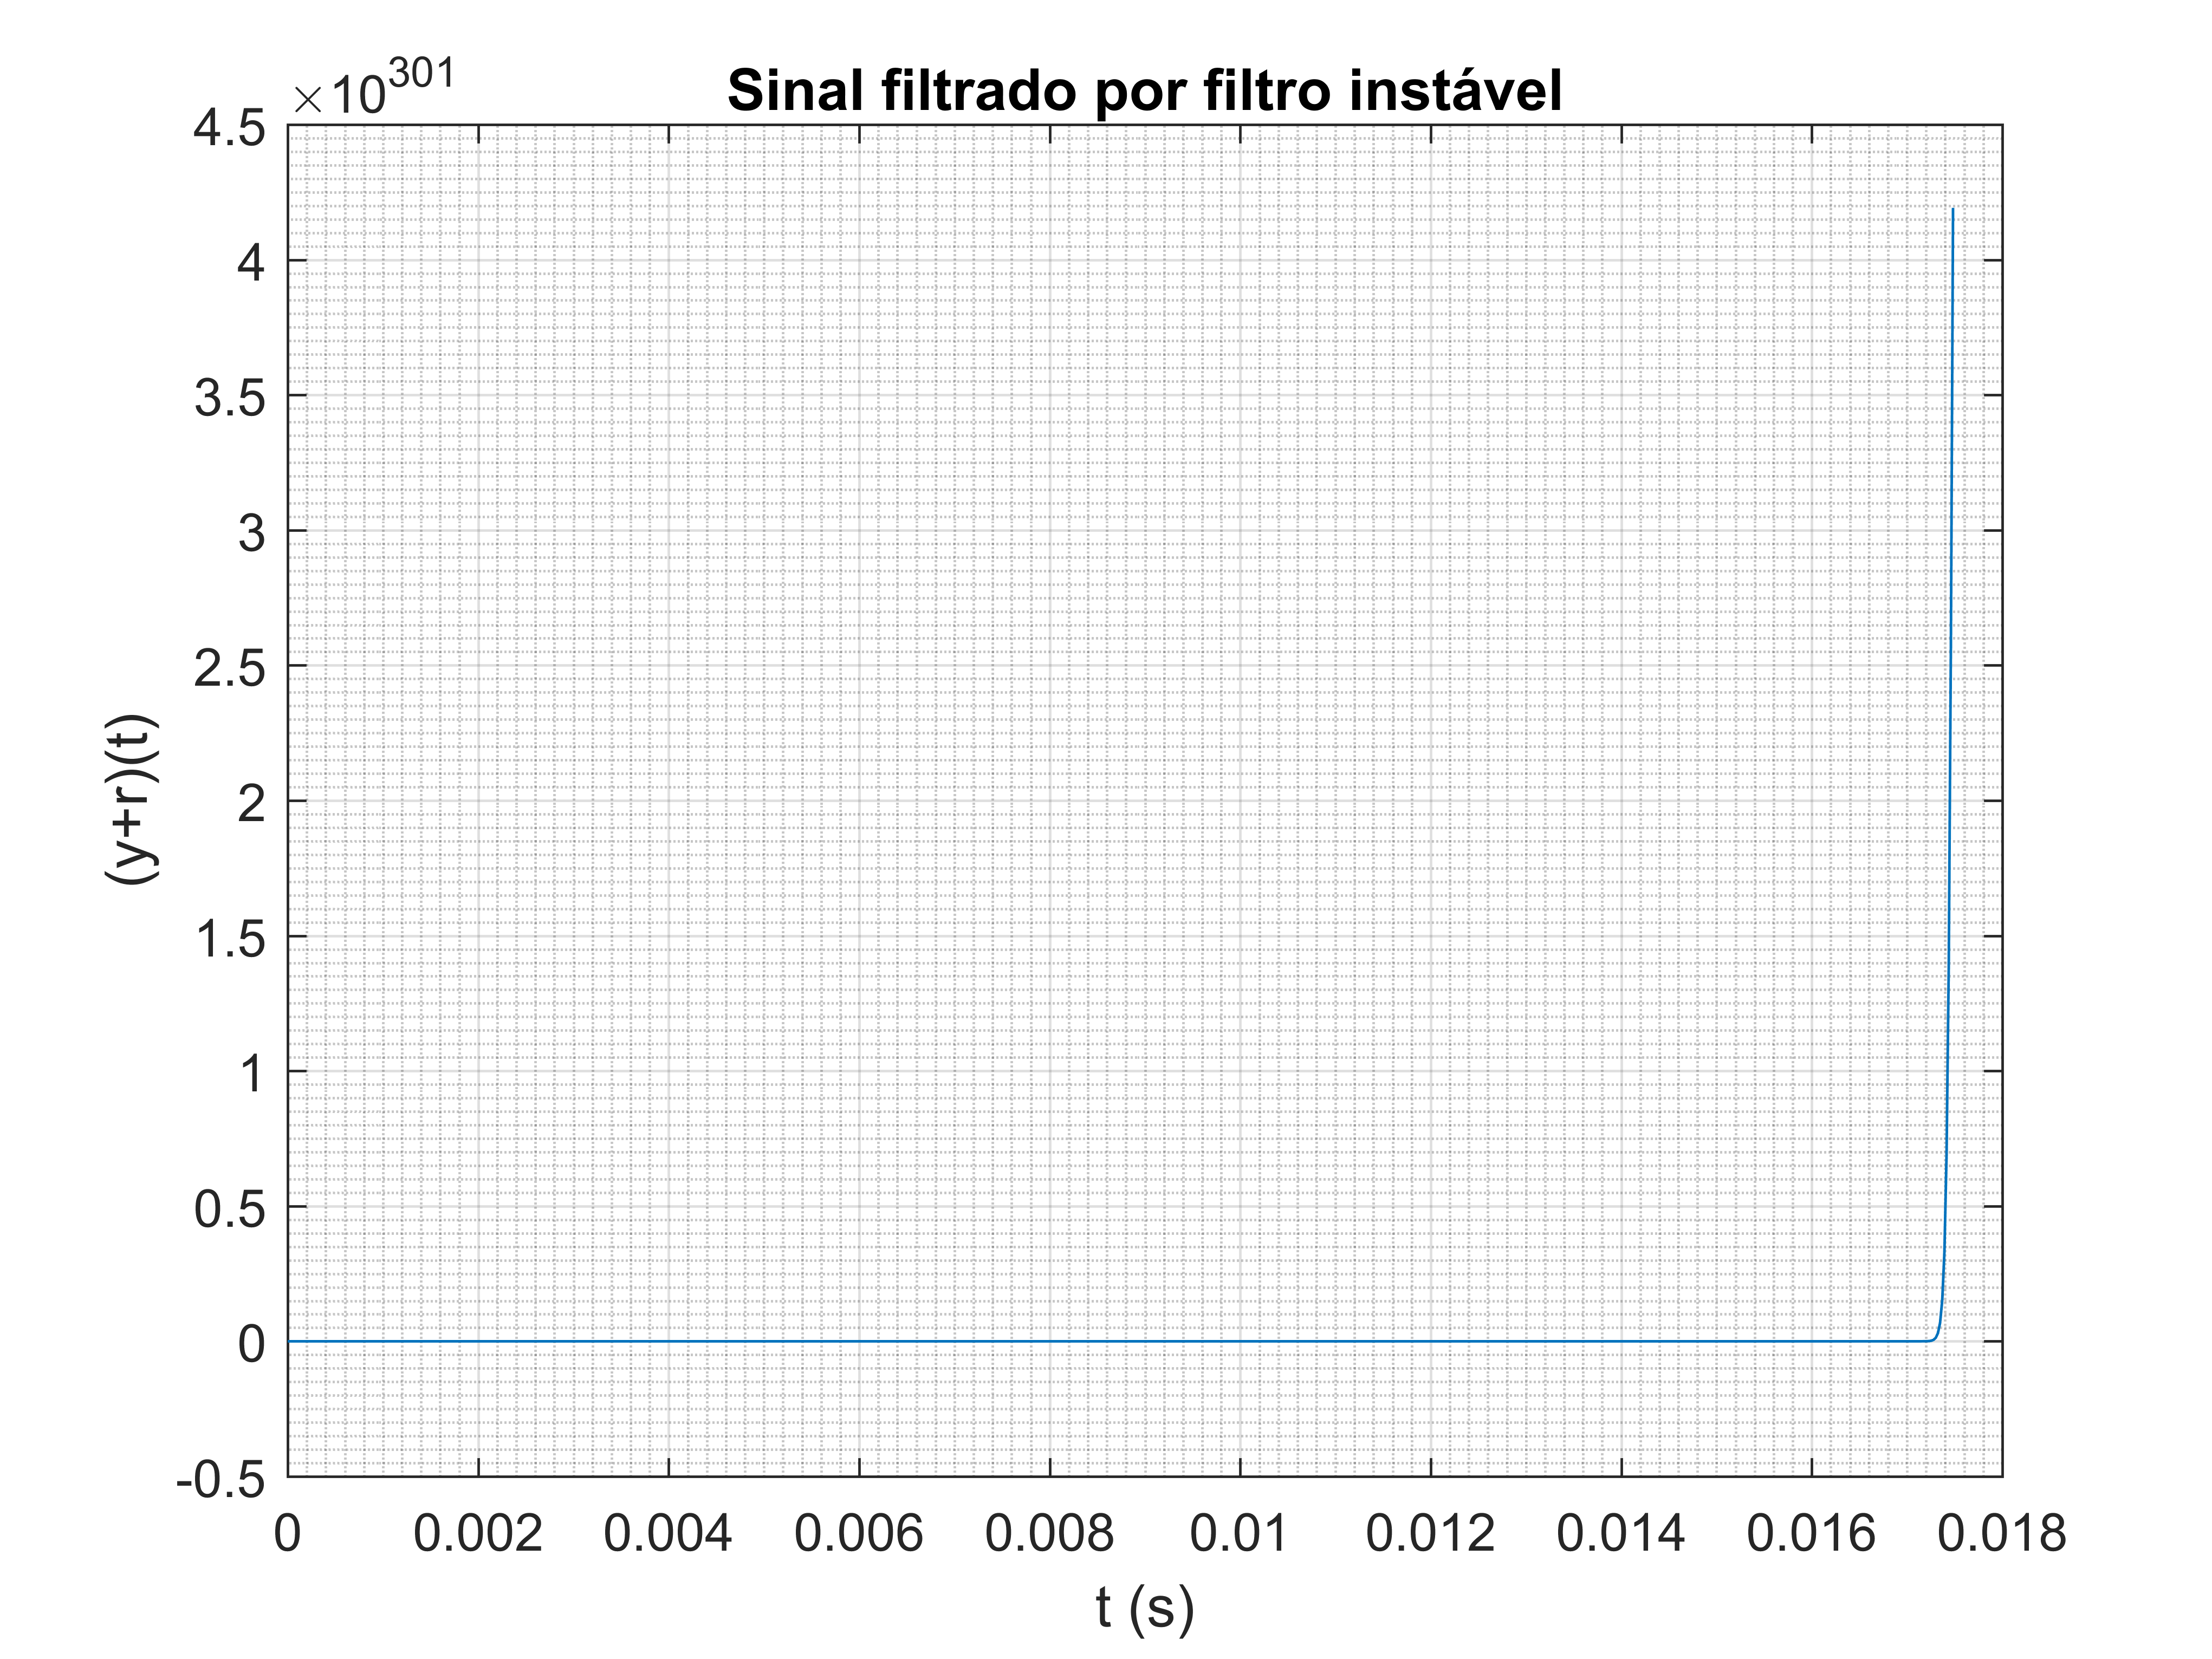
\includegraphics[width=0.6\textwidth]{graficos/filtro_instavel_t.PNG}
    \end{figure} 
    
\end{frame}

\begin{frame}{Tentativa 2 de cálculo de H(s)=N(s)/D(s)}
    Os pólos/zeros do SPD, após discretizados, ficaram fora do círculo unitário e a resposta em fase e magnitude teve comportamento totalmente diferente do desejado para um rejeita-faixa
    \begin{figure}[!htb]
    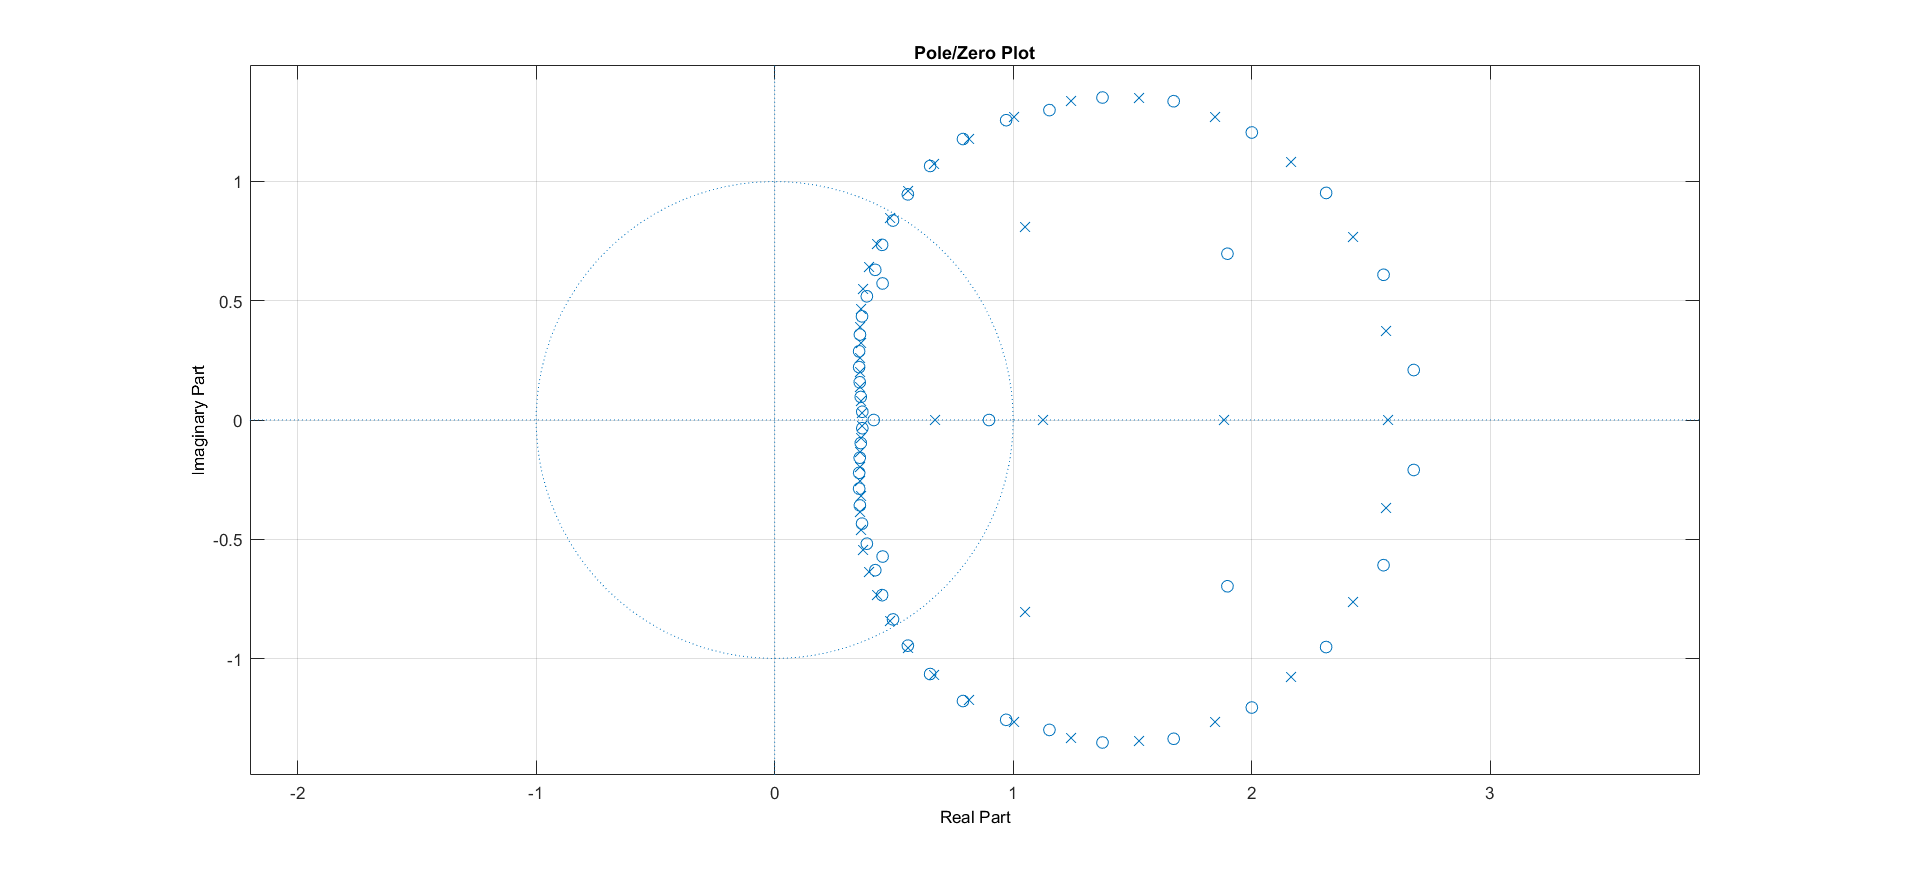
\includegraphics[width=0.9\textwidth]{graficos/zp_b_inst.PNG}
    \end{figure} 
\end{frame}
\begin{frame}{Tentativa 2 de cálculo de H(s)=N(s)/D(s)}
    \begin{figure}[!htb]
    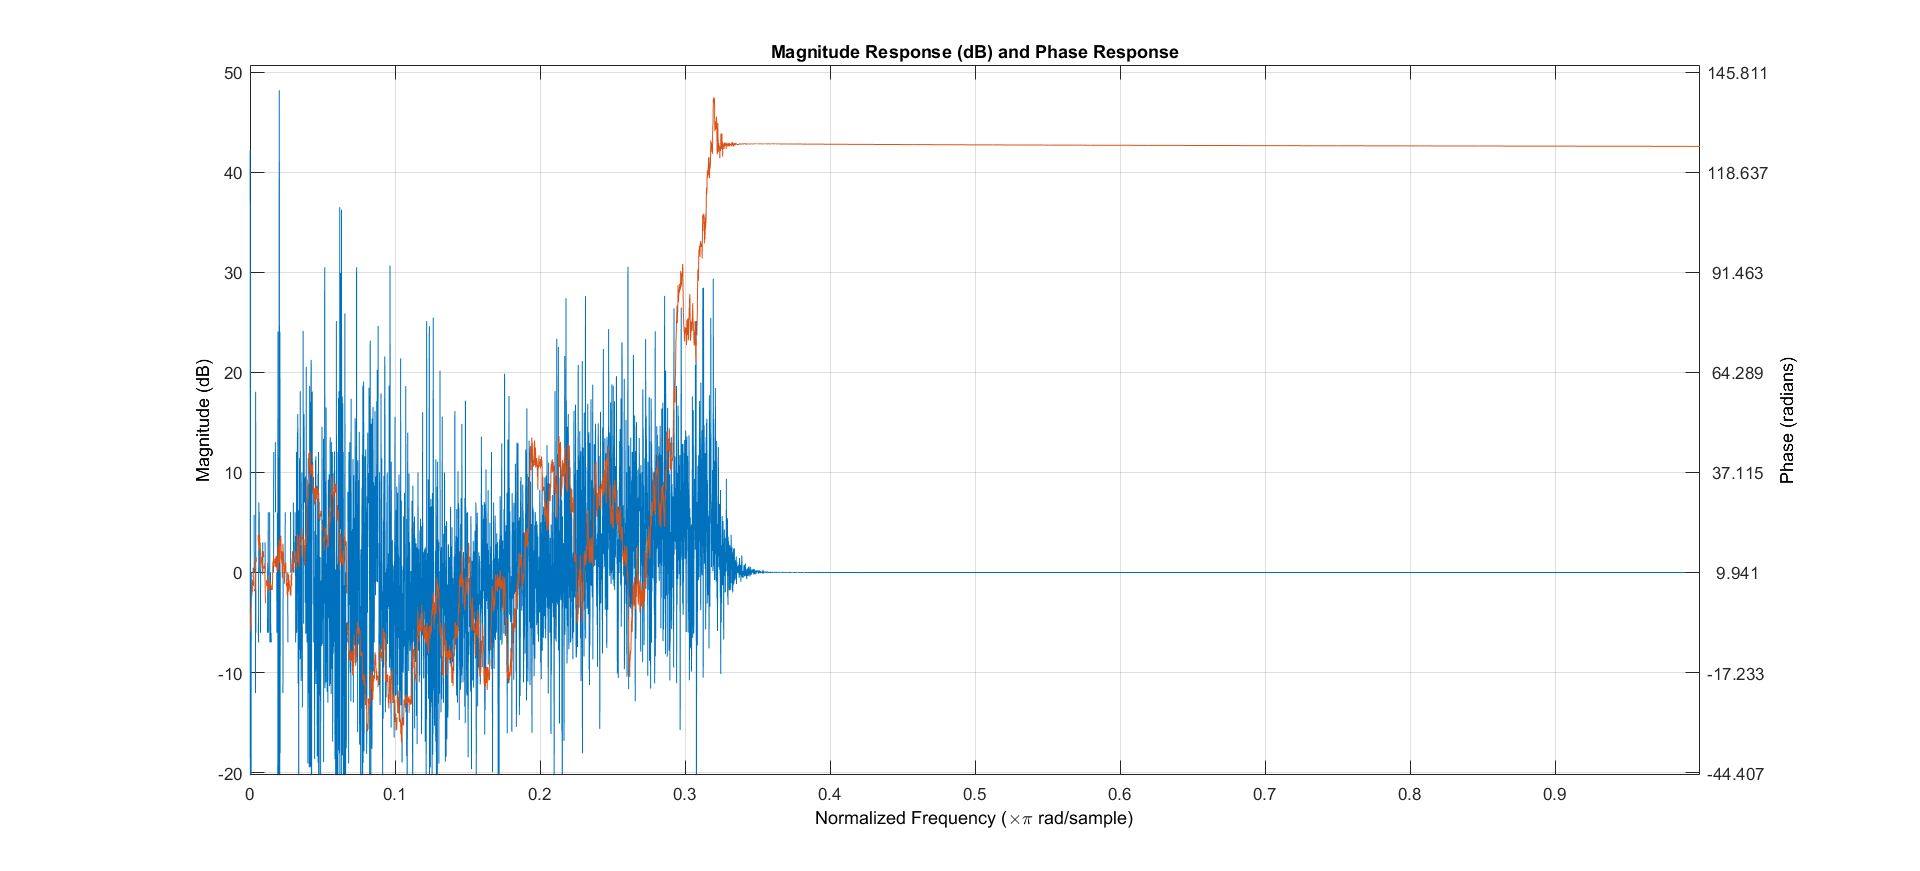
\includegraphics[width=0.9\textwidth]{graficos/mag_pha_b_inst.PNG}
    \end{figure} 
\end{frame}

\begin{frame}{Mitigação de Erro Numérico}
    \begin{itemize}
        \item Noutou-se que ordens altas de polinômios em funções de transferência são suceptíveis a erros númericos
        \item Polos/zeros podem deixar de ser estáveis/fase-mínima
        \item Contornou-se isto com cascatas de sistemas de segunda ordem
        \item O MATLAB usa as SOS (second order sections)
        \item sosfilt(SOS,X) é análoga ao filt(NUM,DEN,Ts) para SOS
    \end{itemize}

\end{frame}

\begin{frame}{Mitigação de Erro Numérico}
    \begin{figure}[!htb]
    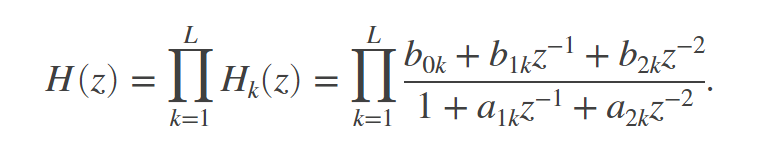
\includegraphics[width=0.6\textwidth]{graficos/eq_sos.PNG}
    \end{figure} 
	\begin{figure}[!htb]
    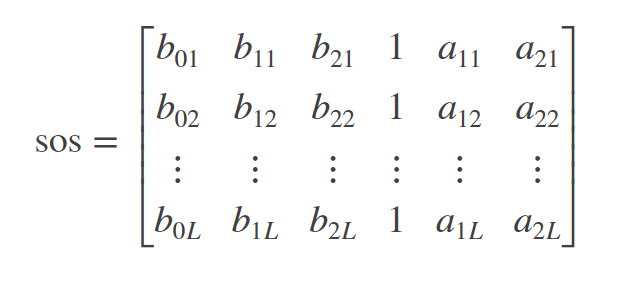
\includegraphics[width=0.6\textwidth]{graficos/matriz_sos.PNG}
    \end{figure} 
\end{frame}

\begin{frame}{Mitigação de Erro Numérico}
    \begin{figure}[!htb]
    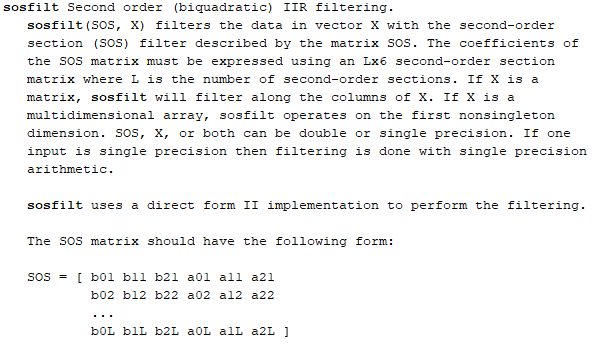
\includegraphics[width=0.9\textwidth]{graficos/sos_filt_doc.png}
    \end{figure}
    
\end{frame}

\begin{frame}{Butterworth e Chebyshev I}
    \begin{figure}[!htb]
    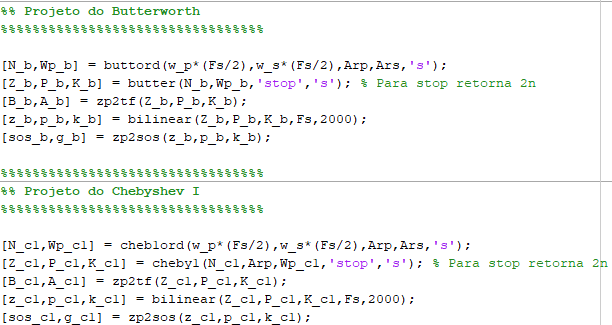
\includegraphics[width=0.9\textwidth]{graficos/code_butt_chebI.PNG}
    \end{figure} 
\end{frame}


\begin{frame}{Chebyshev II e Elíptico}
    \begin{figure}[!htb]
    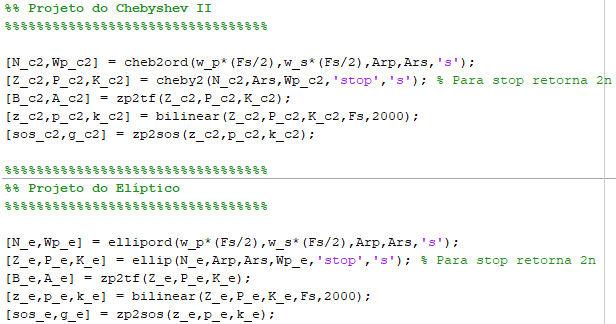
\includegraphics[width=0.9\textwidth]{graficos/code_chebII_ellip.png}
    \end{figure} 
\end{frame}


\begin{frame}{Filtragem das SOS calculadas}
    \begin{figure}[!htb]
    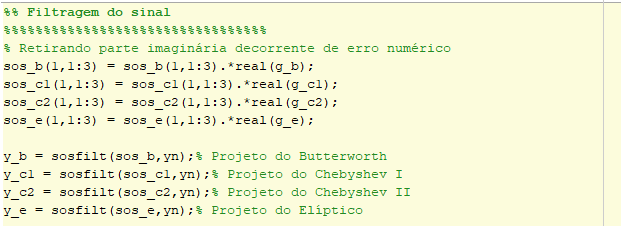
\includegraphics[width=0.9\textwidth]{graficos/code_sos_filtros.png}
    \end{figure} 
\end{frame}